%%%%%%%%%%%%%%%%%%%%%%%%%%%%%%%%%%%%%%%%%%%%%%%%%%%%%%%%%%%%%%%%%%%%%%%%%%%%%%%
% File: sansdir-report.tex
% Technical report describing the sansdir terminal application.
% Built on the ORNL report template (ornltm.cls) supplied in this directory.
%
% Build:  pdflatex sansdir-report
%         biber   sansdir-report
%         pdflatex sansdir-report
%         pdflatex sansdir-report
%%%%%%%%%%%%%%%%%%%%%%%%%%%%%%%%%%%%%%%%%%%%%%%%%%%%%%%%%%%%%%%%%%%%%%%%%%%%%%%
\documentclass[tm]{ornltm}

%% Packages used by this document beyond those loaded by the class.
\usepackage{threeparttable} % Table captions and tablenotes
\usepackage{booktabs}       % Toprule, midrule, bottomrule
\usepackage{multirow}       % Table entries spanning rows
\usepackage{listings}       % Verbatim code blocks
\usepackage{tikz}           % Architecture diagrams
\usetikzlibrary{positioning,arrows.meta,shapes.geometric,fit}

%% Bibliography styling (author-date, per ORNL TM preference).
\usepackage[authordate,autocite=inline,backend=biber,natbib]{biblatex-chicago}
\bibliography{sansdir.bib}

%% Inline small italic blue for editorial comments.
\definecolor{note}{RGB}{48,96,192}
\renewcommand{\marginpar}[1]{{\small\em\color{note}[#1]}}

%% Code-listing style. Terminal transcripts and source snippets are set in a
%% lightly shaded box so they are visually distinct from tables.
\definecolor{codebg}{RGB}{246,246,246}
\definecolor{coderule}{RGB}{200,200,200}
\definecolor{codecomment}{RGB}{90,120,90}
\lstdefinestyle{sansdir}{
  basicstyle=\ttfamily\footnotesize,
  backgroundcolor=\color{codebg},
  frame=single,
  rulecolor=\color{coderule},
  framesep=4pt,
  xleftmargin=6pt,
  xrightmargin=6pt,
  breaklines=true,
  breakatwhitespace=false,
  postbreak=\mbox{\textcolor{coderule}{$\hookrightarrow$}\space},
  columns=fullflexible,
  keepspaces=true,
  showstringspaces=false,
  commentstyle=\color{codecomment}\itshape,
  aboveskip=8pt,
  belowskip=8pt,
}
\lstset{style=sansdir}
\lstdefinelanguage{shellsession}{
  morecomment=[l]{\#},
  sensitive=true,
}

%% This document sets many long unbreakable typewriter tokens (filesystem paths,
%% dotted command names) in justified text. Without extra stretch the paragraph
%% breaker cannot avoid overfull lines around them.
\emergencystretch=2.5em

%% Shorthand for the many dotted command names in this report.
\newcommand{\cmd}[1]{\texttt{#1}}
%% Shorthand for a key cap.
\newcommand{\key}[1]{\textbf{\texttt{#1}}}
%% Home-directory tilde that does not look like a diacritic.
\newcommand{\hme}{\raisebox{0.4ex}{\texttildelow}}

%%%%%%%%%%%%%%%%%%%%%%%%%%%%%%%%%%%%%%%%%%%%%%%%%%%%%%%%%%%%%%%%%%%%%%%%%%%%%%%
% AUTHORSHIP & PUBLISHING
%%%%%%%%%%%%%%%%%%%%%%%%%%%%%%%%%%%%%%%%%%%%%%%%%%%%%%%%%%%%%%%%%%%%%%%%%%%%%%%

\author{Changwoo Do}

\title{SansDIR: A Keyboard-Driven Terminal Application for\\
Navigating, Inspecting, and Plotting\\
Small-Angle Neutron Scattering Data}

\date{\today}

%% NOTE: replace with the number issued by the RESolution Publications system.
\reportnum{ORNL/TM-20XX/XXXX}

\division{Neutron Scattering Division}

%% Remove \reportdraft for public release and unlimited distribution.
\reportdraft

%%%%%%%%%%%%%%%%%%%%%%%%%%%%%%%%%%%%%%%%%%%%%%%%%%%%%%%%%%%%%%%%%%%%%%%%%%%%%%%
% ABBREVIATIONS
%%%%%%%%%%%%%%%%%%%%%%%%%%%%%%%%%%%%%%%%%%%%%%%%%%%%%%%%%%%%%%%%%%%%%%%%%%%%%%%

%%%%%%%%%%%%%%%%%%%%%%%%%%%%%%%%%%%%%%%%%%%%%%%%%%%%%%%%%%%%%%%%%%%%%%%%%%%%%%%
% ABBREVIATIONS -- sansdir technical report
%%%%%%%%%%%%%%%%%%%%%%%%%%%%%%%%%%%%%%%%%%%%%%%%%%%%%%%%%%%%%%%%%%%%%%%%%%%%%%%
%% Uses the Acro package called in the CLS and styled in the STY. Acronyms that
%% are never used in the document are not printed in the List of Abbreviations.
%%%%%%%%%%%%%%%%%%%%%%%%%%%%%%%%%%%%%%%%%%%%%%%%%%%%%%%%%%%%%%%%%%%%%%%%%%%%%%%

%%% ---------------------------------------------------------------- Institutional
\DeclareAcronym{doe}{
  short = DOE ,
  long = US Department of Energy
}

\DeclareAcronym{ornl}{
  short = ORNL ,
  long = Oak Ridge National Laboratory
}

\DeclareAcronym{sns}{
  short = SNS ,
  long = Spallation Neutron Source
}

\DeclareAcronym{hfir}{
  short = HFIR ,
  long = High Flux Isotope Reactor
}

\DeclareAcronym{tm}{
  short = TM ,
  long = Technical Memo
}

%%% ------------------------------------------------------------------ Scientific
\DeclareAcronym{sans}{
  short = SANS ,
  long = small-angle neutron scattering
}

\DeclareAcronym{usans}{
  short = USANS ,
  long = ultra-small-angle neutron scattering
}

\DeclareAcronym{ipts}{
  short = IPTS ,
  long = Integrated Proposal Tracking System
}

\DeclareAcronym{das}{
  short = DAS ,
  long = data acquisition system
}

%%% ------------------------------------------------------------ Software computing
\DeclareAcronym{tui}{
  short = TUI ,
  long = terminal user interface
}

\DeclareAcronym{gui}{
  short = GUI ,
  long = graphical user interface
}

\DeclareAcronym{cli}{
  short = CLI ,
  long = command-line interface
}

\DeclareAcronym{api}{
  short = API ,
  long = application programming interface
}

\DeclareAcronym{hdf}{
  short = HDF5 ,
  long = Hierarchical Data Format version 5
}

\DeclareAcronym{ssh}{
  short = SSH ,
  long = Secure Shell
}

\DeclareAcronym{nfs}{
  short = NFS ,
  long = Network File System
}

\DeclareAcronym{csv}{
  short = CSV ,
  long = comma-separated values
}

\DeclareAcronym{tsv}{
  short = TSV ,
  long = tab-separated values
}

\DeclareAcronym{toml}{
  short = TOML ,
  long = Tom's Obvious Minimal Language
}

\DeclareAcronym{json}{
  short = JSON ,
  long = JavaScript Object Notation
}

\DeclareAcronym{rest}{
  short = REST ,
  long = representational state transfer
}

\DeclareAcronym{llm}{
  short = LLM ,
  long = large language model
}

\DeclareAcronym{ci}{
  short = CI ,
  long = continuous integration
}

\DeclareAcronym{doi}{
  short = DOI ,
  long = digital object identifier
}

\DeclareAcronym{ttl}{
  short = TTL ,
  long = time to live
}

\DeclareAcronym{oauth}{
  short = OAuth2 ,
  long = Open Authorization version 2
}

\DeclareAcronym{png}{
  short = PNG ,
  long = Portable Network Graphics
}

\DeclareAcronym{xml}{
  short = XML ,
  long = Extensible Markup Language
}

\DeclareAcronym{mc}{
  short = mc ,
  long = Midnight Commander
}


%%%%%%%%%%%%%%%%%%%%%%%%%%%%%%%%%%%%%%%%%%%%%%%%%%%%%%%%%%%%%%%%%%%%%%%%%%%%%%%
% FRONT MATTER
%%%%%%%%%%%%%%%%%%%%%%%%%%%%%%%%%%%%%%%%%%%%%%%%%%%%%%%%%%%%%%%%%%%%%%%%%%%%%%%
\begin{document}
\frontmatter

\tableofcontents
\listoffigures
\listoftables
\printacronyms

%%%%%%%%%%%%%%%%%%%%%%%%%%%%%%%%%%%%%%%%%%%%%%%%%%%%%%%%%%%%%%%%%%%%%%%%%%%%%%%
\begin{foreword}

This report documents \textbf{sansdir}, a terminal application developed in the
Neutron Scattering Division at \ac{ornl} to support the day-to-day data-handling
work of \ac{sans} instrument scientists and users. The software is in production
use for \ac{sns} \ac{sans} workflows and is installed on the analysis cluster at
\texttt{/SNS/EQSANS/shared/script/sansdir}.

The report is written for two audiences. Sections~\ref{sec:intro}
through~\ref{sec:config} are a user manual: they describe what the program does,
how to install and run it, and how each feature behaves. Sections
\ref{sec:formats} through \ref{sec:future} are a developer and reviewer
reference: they document the internal architecture, the testing strategy, and
measured performance. Readers who
only want to use the program can stop after Section~\ref{sec:config}; the
appendices provide condensed reference tables of every command and key binding.

\end{foreword}

%%%%%%%%%%%%%%%%%%%%%%%%%%%%%%%%%%%%%%%%%%%%%%%%%%%%%%%%%%%%%%%%%%%%%%%%%%%%%%%
% ABSTRACT
%%%%%%%%%%%%%%%%%%%%%%%%%%%%%%%%%%%%%%%%%%%%%%%%%%%%%%%%%%%%%%%%%%%%%%%%%%%%%%%
\mainmatter
\begin{abstract}

\Ac{sans} users at the \ac{sns} spend a substantial fraction of their beam-time
and post-experiment effort on tasks that are neither data reduction nor data
analysis: locating runs across \ac{ipts} directories, triaging reduced data by
inspecting plots, reading instrument logs out of NeXus files, exporting selected
metadata to tables, and packaging results for collaborators. These tasks are
performed over \ac{ssh} on the analysis cluster, where \ac{gui} tools that
require X11 forwarding respond slowly.

This report describes \textbf{sansdir}, a dual-pane, keyboard-driven \ac{tui}
that consolidates these tasks into a single application requiring no display
server. The program follows the interaction model of the MDIR and Norton
Commander file managers: two independent directory panes, function-key actions,
and file operations that default to moving data from the active pane to the
opposite one. It adds \ac{sans}-specific capability: automatic classification and
plotting of reduced one- and two-dimensional data, detector heat maps computed
directly from raw NeXus event files without a Mantid runtime, a searchable
\ac{hdf} tree browser, batch metadata extraction to \ac{csv} and \ac{tsv}, an
interactive detector-mask editor whose output is compatible with the
\texttt{drtsans} reduction pipeline, and catalog search through the \ac{ornl}
OnCat service.

The central architectural decision is that every user-facing action is a typed
command in a single registry. Key bindings, the interactive command line, and
the non-interactive \ac{cli} are all thin callers of that registry, which makes
the interaction surface uniform, self-documenting, and testable, and which
positions a future natural-language layer as an additional caller rather than a
rewrite. The implementation is approximately 14,100 lines of Python across 56
modules, covered by 530 automated tests, and starts in about 54~ms.

\end{abstract}

%%%%%%%%%%%%%%%%%%%%%%%%%%%%%%%%%%%%%%%%%%%%%%%%%%%%%%%%%%%%%%%%%%%%%%%%%%%%%%%
% 1. INTRODUCTION
%%%%%%%%%%%%%%%%%%%%%%%%%%%%%%%%%%%%%%%%%%%%%%%%%%%%%%%%%%%%%%%%%%%%%%%%%%%%%%%
\acresetall
\section{INTRODUCTION}
\label{sec:intro}

\subsection{MOTIVATION}

A \ac{sans} experiment at the \ac{sns} produces raw event-mode NeXus files, one
per run, that are written into an \ac{ipts} directory tree of the form
\texttt{/SNS/EQSANS/IPTS-NNNNN/nexus/}. Reduction---performed by
\texttt{drtsans} \autocite{drtsans} or by the automatic reduction service---emits
one-dimensional $I(q)$ profiles, two-dimensional $I(q_x,q_y)$ arrays,
transmission curves, and log files into a parallel \texttt{shared/} tree. A
single proposal routinely accumulates hundreds of runs and several thousand
derived files.

Between measurement and publication, the instrument scientist and the user
perform a set of tasks that are repetitive, unglamorous, and poorly served by
existing software:

\begin{itemize}
  \item \textbf{Navigation.} Moving between \ac{ipts} directories, between the
    \texttt{nexus/} and \texttt{shared/} subtrees of one proposal, and between a
    proposal directory and a personal scratch area.
  \item \textbf{Triage.} Opening a reduced $I(q)$ file to check whether a
    measurement worked, comparing two or three curves on the same axes, or
    looking at a raw detector image to confirm beam-center and beam-stop
    placement.
  \item \textbf{Log inspection.} Reading sample environment values---temperature,
    shear rate, sample position---out of the \ac{das} logs stored inside a NeXus
    file, either for one run or as a table across many runs.
  \item \textbf{Packaging.} Selecting a subset of results, compressing them, and
    emailing them to a collaborator.
\end{itemize}

None of these is difficult in isolation. What makes them costly is that they are
performed dozens of times a day, from a terminal session on the analysis cluster,
and that the available tools each address only one of them. Mantid Workbench
\autocite{mantid} is a full analysis environment and is correspondingly heavy to
launch for the purpose of glancing at one curve. A file manager handles
navigation but knows nothing about \ac{sans} file formats. Reading \ac{das} logs
means writing a short \texttt{h5py} \autocite{h5py} script. Any \ac{gui} tool
launched over \ac{ssh} with X11 forwarding responds with a latency that makes
rapid iteration unpleasant.

The economic argument for \textbf{sansdir} is therefore not that it does
something impossible, but that it collapses a dozen context switches per hour
into a single keyboard-driven application that runs natively in the terminal the
scientist is already using.

\subsection{DESIGN PRINCIPLES}
\label{sec:principles}

Four principles govern the implementation. They are recorded here because they
are binding on future contributions, not merely descriptive.

\begin{enumerate}
  \item \textbf{Speed first.} Every interaction must feel instantaneous. No
    blocking input/output is permitted on the user-interface thread; catalog
    queries, \ac{hdf} reads, and plot rendering run on worker threads or in
    separate processes.
  \item \textbf{Keyboard-driven.} Every action has a single-key or short-chord
    binding. Mouse support is acceptable but never required.
  \item \textbf{Predictable.} A user familiar with MDIR, Norton Commander, or
    \ac{mc}-style file managers \autocite{midnightcommander} should be productive
    within minutes. This dictates two panes, function-key actions, and
    ``operate from the active pane into the opposite pane'' semantics.
  \item \textbf{The command registry is the single source of truth.} Every
    user-facing action is a registered command with a name, typed parameters, a
    description, and examples. Key bindings, the command line, and the \ac{cli}
    all dispatch through it. No key handler is ever wired directly to
    business logic.
\end{enumerate}

\subsection{HERITAGE AND RELATED TOOLS}

The interaction model descends from MDIR, a DOS-era file manager, and from the
Norton Commander family that includes \ac{mc}. The defining feature of that
family is the dual-pane layout: two independent directory views, exactly one of
which is active, with copy and move operations defaulting to ``from the active
pane to the other pane.'' This convention eliminates the source-and-destination
dialog that dominates single-pane and graphical file managers, and it is the
reason experienced Norton Commander users move files faster than mouse-driven
equivalents. Preserving it is treated as a hard constraint rather than an
aesthetic preference.

\textbf{sansdir} is complementary to, not a replacement for, the existing
\ac{sns} software stack. It performs no data reduction; \texttt{drtsans} remains
the reduction engine. It performs no model fitting. It does not replace Mantid
Workbench for interactive analysis. Its scope is deliberately the layer
\emph{around} reduction and analysis: finding files, looking at them, extracting
metadata from them, and moving them. Where the boundary is crossed---the
detector-mask editor of Section~\ref{sec:mask} produces an input to
reduction---the output format is defined by what \texttt{drtsans} consumes.

An earlier tool by the same author, \texttt{eqsanscli} \autocite{eqsanscli},
provided command-line access to OnCat catalog search. Its \ac{api} endpoints and
authentication flow informed the OnCat client described in
Section~\ref{sec:oncat}, which was reimplemented rather than vendored.

\subsection{SCOPE OF THIS REPORT}

This report describes version 0.9.0. Section~\ref{sec:install} covers
installation and deployment. Section~\ref{sec:arch} describes the software
architecture, with emphasis on the command registry. Sections~\ref{sec:ui}
through~\ref{sec:mask} document the user-facing feature set. Section~\ref{sec:cli}
covers non-interactive use, and Section~\ref{sec:config} the configuration file.
Sections~\ref{sec:formats} through~\ref{sec:perf} cover the supported data
formats, the test suite, and measured performance. Section~\ref{sec:future}
summarizes the work and states the limitations that bound it.

%%%%%%%%%%%%%%%%%%%%%%%%%%%%%%%%%%%%%%%%%%%%%%%%%%%%%%%%%%%%%%%%%%%%%%%%%%%%%%%
% 2. INSTALLATION
%%%%%%%%%%%%%%%%%%%%%%%%%%%%%%%%%%%%%%%%%%%%%%%%%%%%%%%%%%%%%%%%%%%%%%%%%%%%%%%
\section{INSTALLATION AND DEPLOYMENT}
\label{sec:install}

\subsection{ZERO-INSTALL DEPLOYMENT ON THE ANALYSIS CLUSTER}

The primary deployment target is the \ac{ornl} analysis cluster, where the
repository is installed at \texttt{/SNS/EQSANS/shared/script/sansdir} together
with a self-contained Python virtual environment. Every cluster user has read
access to that path, so no per-user installation step is required:

\begin{lstlisting}[language=shellsession]
/SNS/EQSANS/shared/script/sansdir/bin/sansdir
/SNS/EQSANS/shared/script/sansdir/bin/sansdir /SNS/EQSANS/IPTS-12345/shared
\end{lstlisting}

To avoid typing the full path, users are advised to create a symbolic link in a
directory already on their \texttt{PATH}. On the analysis nodes both
\texttt{\hme/bin} and \texttt{\hme/.local/bin} are on the default \texttt{PATH}:

\begin{lstlisting}[language=shellsession]
mkdir -p ~/bin
ln -s /SNS/EQSANS/shared/script/sansdir/bin/sansdir ~/bin/sansdir
sansdir --version
\end{lstlisting}

Alternatively, the shared \texttt{bin} directory can be prepended to
\texttt{PATH} in the user's shell profile.

\subsection{PORTABILITY OF THE LAUNCHER}

The entry-point script may also simply be copied anywhere on the filesystem and
executed from there. This works because the script's shebang line names an
\emph{absolute} interpreter path inside the shared virtual environment, so the
kernel executes the bundled Python regardless of where the script file itself
resides. The resulting execution chain is:

\begin{lstlisting}
[user's copy of the script]
  -> /gpfs/.../sansdir/.venv/bin/python      (via absolute shebang)
     -> /gpfs/.../sansdir/src/sansdir/cli.py  (via the venv's editable install)
\end{lstlisting}

Two consequences follow. First, the copy is independent of the user's active
conda environment, current working directory, and whichever Python happens to be
first on \texttt{PATH}. Second, a \emph{symbolic link is preferable to a copy}
in practice: when the shared environment is rebuilt, every user holding a symlink
picks up the new build automatically, whereas holders of copies do not.

Table~\ref{tab:portable} summarizes which components must remain on the shared
mount and which are freely relocatable.

\begin{table}[ht]
  \centering
  \caption{Relocatable and fixed components of a shared installation}
  \label{tab:portable}
  \small
  \begin{tabular}{p{0.42\textwidth} p{0.13\textwidth} p{0.36\textwidth}}
    \toprule
    Path & Status & Note \\
    \midrule
    \texttt{.venv/} & Fixed & Bundled Python interpreter and dependencies. \\
    \texttt{src/sansdir/} & Fixed & Source tree that the editable install
      points to. \\
    \texttt{.venv/bin/sansdir} & Portable & Python entry point; shebang is
      absolute. \\
    \texttt{bin/sansdir} & Portable & Shell launcher; self-locates relative to
      the shared root. \\
    \bottomrule
  \end{tabular}
\end{table}

\subsection{DEPENDENCIES}

Python 3.10 or newer is required. Table~\ref{tab:deps} lists the runtime
dependencies and the role each plays. The dependency set is deliberately small;
proposals to add libraries---in particular \texttt{pandas}, \texttt{scipy}, or
any character-cell plotting library---require justification against the startup
budget of Section~\ref{sec:startup}.

\begin{table}[ht]
  \centering
  \begin{threeparttable}
  \caption{Runtime dependencies}
  \label{tab:deps}
  \small
  \begin{tabular}{l l p{0.52\textwidth}}
    \toprule
    Package & Minimum & Role \\
    \midrule
    \texttt{textual}    & 0.80  & \Ac{tui} framework; asynchronous, themeable
      \autocite{textual}. \\
    \texttt{click}      & 8.1   & \Ac{cli} subcommand dispatch
      \autocite{click}. \\
    \texttt{matplotlib} & 3.7   & All plotting \autocite{matplotlib}. \\
    \texttt{numpy}      & 1.24  & Array input/output for ASCII and NeXus data
      \autocite{numpy}. \\
    \texttt{h5py}       & 3.9   & NeXus and \ac{hdf} access \autocite{h5py}. \\
    \texttt{httpx}      & 0.27  & Asynchronous \ac{rest} client for OnCat. \\
    \texttt{send2trash} & 1.8   & Recoverable delete, with a fallback for
      cluster filesystems that provide no trash directory. \\
    \texttt{tomli}      & 2.0   & \Ac{toml} parsing on Python 3.10 only;
      Python 3.11 and newer use the standard-library \texttt{tomllib}. \\
    \bottomrule
  \end{tabular}
  \begin{tablenotes}
    \item \emph{Note:} Optional extras are \texttt{qt} (installs PyQt5 for an
    interactive matplotlib backend), \texttt{tk} (a marker extra; the
    \texttt{tkinter} module ships with most Python builds), \texttt{llm} (the
    Anthropic client for the planned natural-language layer), and \texttt{dev}.
  \end{tablenotes}
  \end{threeparttable}
\end{table}

\subsection{VERIFYING AN INSTALLATION}

\begin{lstlisting}[language=shellsession]
sansdir --version           # prints the version and exits
sansdir --help              # subcommands and worked examples
sansdir extract --help      # per-subcommand help
\end{lstlisting}

A successful \texttt{--version} invocation confirms that the interpreter,
package, and entry point resolve correctly. It deliberately does not import
Textual, matplotlib, or \texttt{h5py}, so it also serves as a check that the
lazy-import discipline of Section~\ref{sec:startup} is intact.

%%%%%%%%%%%%%%%%%%%%%%%%%%%%%%%%%%%%%%%%%%%%%%%%%%%%%%%%%%%%%%%%%%%%%%%%%%%%%%%
% 3. ARCHITECTURE
%%%%%%%%%%%%%%%%%%%%%%%%%%%%%%%%%%%%%%%%%%%%%%%%%%%%%%%%%%%%%%%%%%%%%%%%%%%%%%%
\section{SOFTWARE ARCHITECTURE}
\label{sec:arch}

\subsection{LAYERED STRUCTURE}

The program is organized in four layers, shown in Figure~\ref{fig:arch}. Entry
points at the top translate user intent into a command name and arguments. The
command registry in the middle is the sole dispatch mechanism. The service layer
below it contains all business logic, grouped by concern. External resources sit
at the bottom.

\begin{figure}[ht]
  \centering
  \resizebox{\textwidth}{!}{% Layered architecture of sansdir. Included by sansdir-report.tex.
% Requires: \usepackage{tikz} with the positioning, arrows.meta, fit libraries.
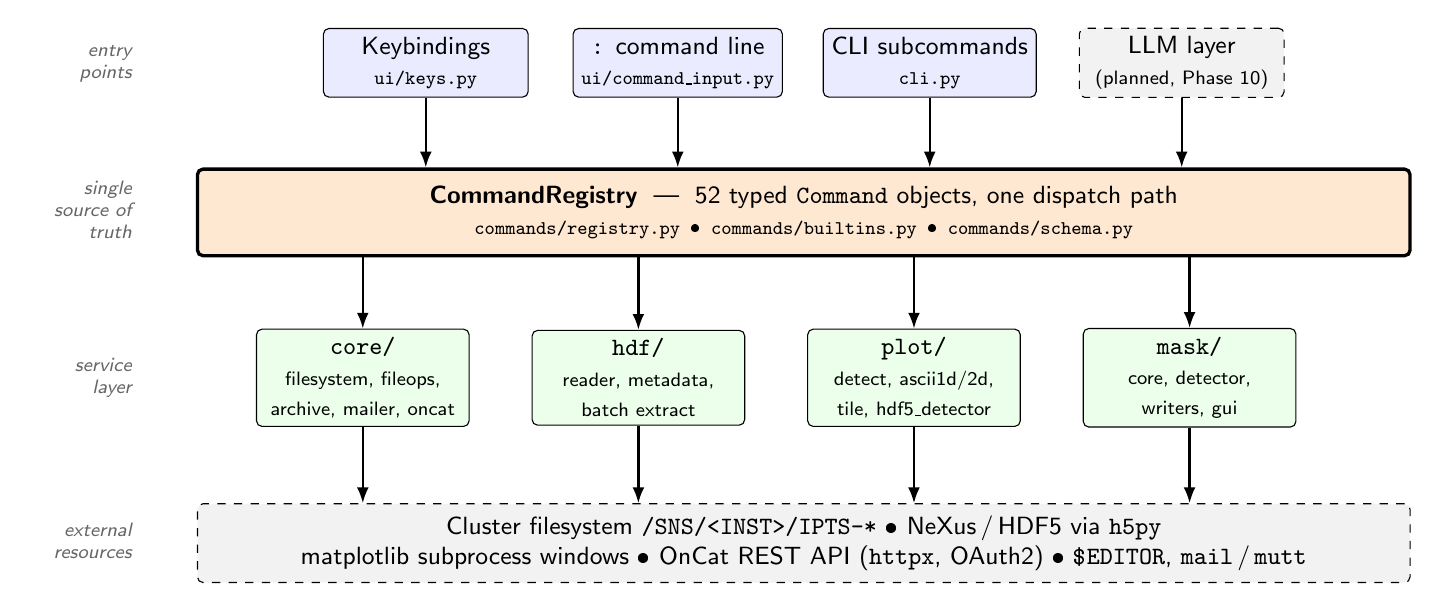
\begin{tikzpicture}[
    font=\small\sffamily,
    box/.style={draw, rounded corners=2pt, minimum height=8mm, align=center,
                inner sep=3pt},
    ui/.style={box, fill=blue!8},
    reg/.style={box, fill=orange!18, very thick},
    svc/.style={box, fill=green!8},
    ext/.style={box, fill=gray!10, dashed},
    lbl/.style={font=\scriptsize\sffamily\itshape, text=black!60},
    flow/.style={-{Latex[length=2mm]}, thick},
  ]

  % --- Entry points -------------------------------------------------------
  \node[ui, minimum width=26mm] (keys)  at (-4.6, 5.2) {Keybindings\\\scriptsize\ttfamily ui/keys.py};
  \node[ui, minimum width=26mm] (cmdl)  at (-1.4, 5.2) {\texttt{:} command line\\\scriptsize\ttfamily ui/command\_input.py};
  \node[ui, minimum width=26mm] (cli)   at ( 1.8, 5.2) {CLI subcommands\\\scriptsize\ttfamily cli.py};
  \node[ext, minimum width=26mm] (llm)  at ( 5.0, 5.2) {LLM layer\\\scriptsize (planned, Phase 10)};

  \node[lbl, anchor=east] at (-8.0, 5.2) {\begin{tabular}{r}entry\\points\end{tabular}};

  % --- Registry -----------------------------------------------------------
  \node[reg, minimum width=15.4cm, minimum height=11mm] (registry) at (0.2, 3.3)
    {\textbf{CommandRegistry} \;---\; 52 typed \texttt{Command} objects, one dispatch path\\
     \scriptsize\ttfamily commands/registry.py \textbullet\ commands/builtins.py \textbullet\ commands/schema.py};

  \node[lbl, anchor=east] at (-8.0, 3.3) {\begin{tabular}{r}single\\source of\\truth\end{tabular}};

  % --- Service layer ------------------------------------------------------
  \node[svc, minimum width=27mm] (core) at (-5.4, 1.2) {\texttt{core/}\\\scriptsize filesystem, fileops,\\\scriptsize archive, mailer, oncat};
  \node[svc, minimum width=27mm] (hdf)  at (-1.9, 1.2) {\texttt{hdf/}\\\scriptsize reader, metadata,\\\scriptsize batch extract};
  \node[svc, minimum width=27mm] (plot) at ( 1.6, 1.2) {\texttt{plot/}\\\scriptsize detect, ascii1d/2d,\\\scriptsize tile, hdf5\_detector};
  \node[svc, minimum width=27mm] (mask) at ( 5.1, 1.2) {\texttt{mask/}\\\scriptsize core, detector,\\\scriptsize writers, gui};

  \node[lbl, anchor=east] at (-8.0, 1.2) {\begin{tabular}{r}service\\layer\end{tabular}};

  % --- External resources -------------------------------------------------
  % One wide band rather than four boxes: several services touch the same
  % resource (mask and hdf both read NeXus), so per-box arrows would cross.
  \node[ext, minimum width=15.4cm, minimum height=10mm] (extern) at (0.2, -0.9)
    {Cluster filesystem \texttt{/SNS/<INST>/IPTS-*} \textbullet\ NeXus\,/\,HDF5 via \texttt{h5py}\\
     matplotlib subprocess windows \textbullet\ OnCat REST API (\texttt{httpx}, OAuth2)
     \textbullet\ \texttt{\$EDITOR}, \texttt{mail}\,/\,\texttt{mutt}};

  \node[lbl, anchor=east] at (-8.0, -0.9) {\begin{tabular}{r}external\\resources\end{tabular}};

  % --- Arrows -------------------------------------------------------------
  \foreach \n in {keys, cmdl, cli, llm}
    \draw[flow] (\n) -- (\n |- registry.north);
  \foreach \n in {core, hdf, plot, mask}
    \draw[flow] (\n |- registry.south) -- (\n);
  \foreach \n in {core, hdf, plot, mask}
    \draw[flow] (\n) -- (\n |- extern.north);

\end{tikzpicture}
}
  \longcaption{Layered architecture of sansdir.}{Every entry point---key
  bindings, the interactive command line, \ac{cli} subcommands, and the planned
  natural-language layer---converges on a single command registry. The
  application shell owns no business logic; the service layer below the registry
  contains all of it.}
  \label{fig:arch}
\end{figure}

The Textual application object owns presentation state only: which pane is
active, what the cursor and tags are, which modal screen is on the stack. It
contains no file, plotting, or catalog logic. This separation is what makes the
service layer testable without instantiating a terminal application, and it is
enforced by code review.

\subsection{THE COMMAND REGISTRY}
\label{sec:registry}

The registry is the most consequential design decision in the project. Every
user-facing action---change directory, tag, copy, plot, extract metadata, search
the catalog, create a mask---is represented as a \texttt{Command} object holding
a dotted name, a one-sentence description, a tuple of typed parameters, a
handler, optional aliases and examples, and a \texttt{danger} flag marking
destructive operations. Parameters are themselves typed objects with a name, a
type drawn from a fixed vocabulary (\texttt{path}, \texttt{glob},
\texttt{string}, \texttt{int}, \texttt{float}, \texttt{bool}, \texttt{enum},
\texttt{files}), a description, a required flag, a default, and---for
enumerations---a list of permitted values.

Validation is performed at construction time and at dispatch time. A parameter
declaring an unknown type, or an enumeration without choices, raises
immediately when the command is built, so a malformed command definition fails
at import rather than when a user first presses the key. At dispatch, unknown
keyword arguments and missing required arguments both raise \texttt{TypeError}
before the handler runs.

Handlers may be synchronous or asynchronous. \texttt{dispatch} is itself
asynchronous and awaits the handler's result if it is awaitable, so callers have
exactly one calling convention regardless of how a particular handler is
implemented. A synchronous convenience wrapper exists for call sites that are not
already inside an event loop; it raises rather than silently misbehaving if
invoked from within one.

Version 0.9.0 registers 52 commands. Appendix~\ref{sec:appcommands} lists them
in full.

\subsection{DISPATCH PATHS}

Four callers use the registry, as summarized in Table~\ref{tab:dispatch}. There
is intentionally no fifth path: no code in the user-interface layer calls a
service function directly.

\begin{table}[ht]
  \centering
  \caption{Callers of the command registry}
  \label{tab:dispatch}
  \small
  \begin{tabular}{p{0.20\textwidth} p{0.72\textwidth}}
    \toprule
    Caller & Path \\
    \midrule
    Key binding &
      \texttt{ui/keys.py} maps \key{F6} to \cmd{ui.copy\_tagged}, resolves the
      active pane's selection and the inactive pane's directory into keyword
      arguments, and dispatches. \\
    Command line &
      \texttt{ui/command\_input.py} parses \texttt{cd /SNS/EQSANS} into the
      command name \cmd{nav.cd} and the argument \texttt{path}, then
      dispatches. \\
    \Ac{cli} &
      \texttt{sansdir extract -k ...} builds arguments and calls the same
      extraction code path used by the interactive dialog. \\
    \Ac{llm} layer &
      Planned. The registry already exports a \ac{json} tool schema; a
      natural-language front end would emit command names with typed arguments,
      display them for confirmation, and dispatch. \\
    \bottomrule
  \end{tabular}
\end{table}

Three properties follow from this discipline, and they are the practical
justification for it. First, the interactive and non-interactive interfaces
cannot drift apart, because they are the same code. Second, the help overlay is
generated from registry metadata rather than maintained by hand, so it cannot
become stale---Figure~\ref{fig:help} shows the generated output. Third, the
future natural-language layer is an additional caller rather than a
reimplementation.

\begin{figure}[ht]
  \centering
  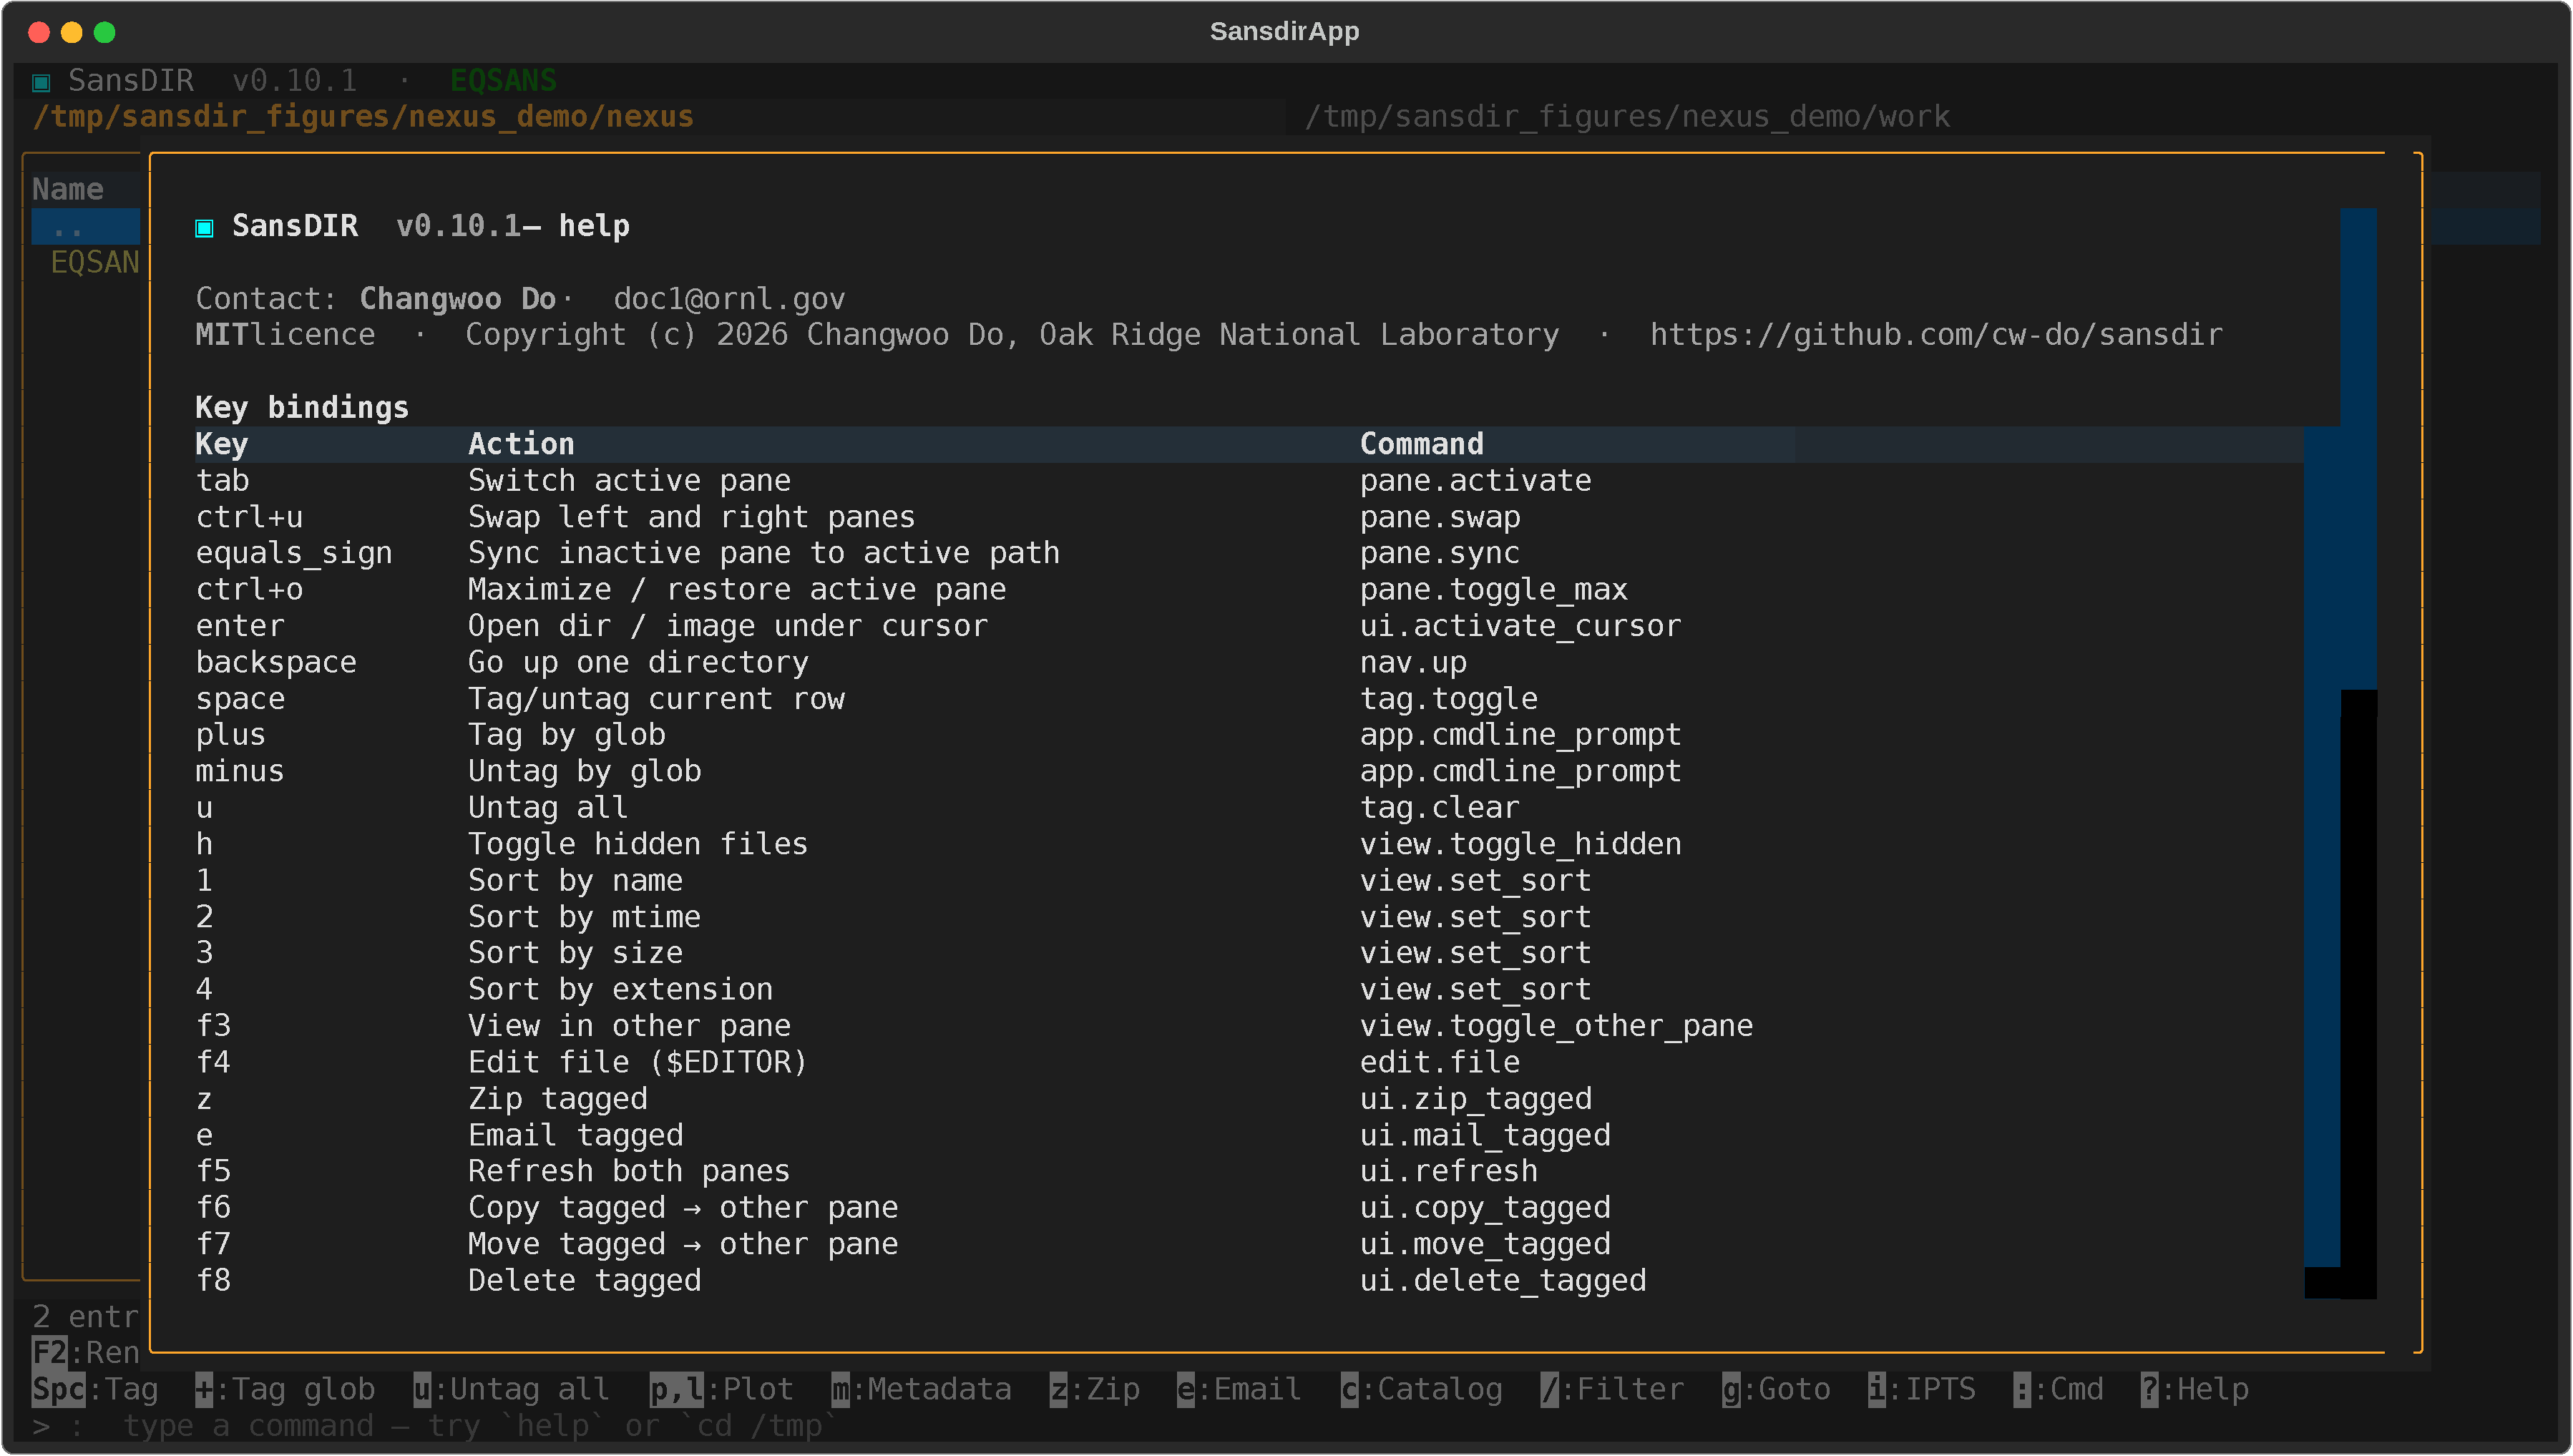
\includegraphics[width=\textwidth]{figures/help-overlay.pdf}
  \longcaption{The help overlay, generated from the registry.}{Each row pairs a
  keystroke with its human-readable action and the underlying command name. The
  third column is what makes the mapping between the two interaction surfaces
  discoverable: any key can be re-issued as a typed command, and any command can
  be rebound to a key.}
  \label{fig:help}
\end{figure}

\subsection{KEY BINDINGS AS DATA}

The key map is a plain list of immutable \texttt{KeyBinding} records, each naming
a key, a command, a description, and an optional \emph{argument resolver}---a
small named function that converts the running application's state into the
keyword arguments the command expects. For example, the resolver bound to
\key{m} extracts the path under the cursor in the active pane and returns it as
the \texttt{path} argument to \cmd{hdf.show\_keys}.

Resolvers are named functions rather than anonymous lambdas so that tracebacks
and the help overlay display meaningful names. The default map contains 48
bindings, of which 38 are shown in the help overlay; the remainder are duplicate
encodings of the same key. Duplicates exist because terminals disagree on how to
report certain keys: the equals sign arrives as \texttt{equals\_sign} on most
terminals and as \texttt{=} on others, so both are registered and the redundant
entry is hidden from help.

A test asserts that every binding names a command that exists in a fully bound
registry, so a typo in the key map fails in \ac{ci} rather than at runtime.

Users may override or extend the map through the \texttt{[keys]} section of the
configuration file. Entries naming an unknown command are dropped at startup with
a notification rather than aborting the launch.

\subsection{THE COMMAND LINE PARSER}

The \key{:} line accepts registered command names and aliases with positional and
keyword arguments. It performs no natural-language interpretation and contains no
\texttt{eval} or \texttt{exec}; this is a deliberate safety boundary, and
natural-language input is reserved for the future \ac{llm} layer, which can emit
only registry-defined commands with typed arguments.

Aliases keep the typed interface terse. \cmd{nav.cd} is reachable as
\texttt{cd}, \cmd{hdf.batch\_extract} as \texttt{extract},
\cmd{oncat.search} as \texttt{ipts}, and \cmd{shell.run} as \texttt{!}.
Command history persists across sessions.

\subsection{STARTUP BUDGET AND LAZY IMPORTS}
\label{sec:startup}

The design budget is 300~ms from invocation to first paint. The measured cold
start for \texttt{sansdir --help} is approximately 54~ms.

This is achieved by importing only \texttt{click} and the version constant at
module scope in the \ac{cli}. Textual, matplotlib, \texttt{h5py}, \texttt{httpx},
and the registry itself are imported inside the subcommand bodies that need them.
The practical effect is that \texttt{sansdir version} and \texttt{sansdir --help}
never pay for the scientific stack, and that the \ac{tui}'s own startup imports
Textual but still defers matplotlib and \texttt{h5py} until the first plot or
metadata operation.

The budget is checked after any change that touches the import graph.

\subsection{CONCURRENCY MODEL}

Three mechanisms keep the interface responsive:

\begin{itemize}
  \item \textbf{Thread offload.} Blocking library calls---principally
    \texttt{h5py} reads---run through \texttt{asyncio.to\_thread}. The \ac{hdf}
    key search of Section~\ref{sec:hdfsearch} is a representative case: walking a
    large raw NeXus file takes seconds, so the walk runs on a thread and the
    result is cached on the screen object for subsequent queries.
  \item \textbf{Textual workers.} Longer interactive operations run as
    background workers so that the event loop continues to service keystrokes.
    The mask editor's launcher, for instance, awaits the editor subprocess in a
    worker and refreshes both panes when it exits with a save.
  \item \textbf{Subprocesses.} Plot windows run in a separate process, which
    is the only reliable way to give matplotlib its own \ac{gui} event loop
    without contending with Textual's.
\end{itemize}

\subsection{REPOSITORY LAYOUT}

Table~\ref{tab:layout} lists the package structure. The implementation totals
approximately 14,100 lines across 56 modules.

\begin{table}[ht]
  \centering
  \caption{Package structure}
  \label{tab:layout}
  \small
  \begin{tabular}{l p{0.68\textwidth}}
    \toprule
    Path & Contents \\
    \midrule
    \texttt{cli.py} & Click entry point; \texttt{tui}, \texttt{extract},
      \texttt{mask}, and \texttt{version} subcommands. \\
    \texttt{app.py} & The Textual application shell. \\
    \texttt{config.py} & \Ac{toml} configuration loader. \\
    \texttt{commands/} & \texttt{registry.py} (the \texttt{Command} model and
      dispatch), \texttt{builtins.py} (all 52 registrations),
      \texttt{parser.py} (the \key{:} line), \texttt{schema.py} (\ac{json} tool
      schema export). \\
    \texttt{core/} & \texttt{filesystem.py} (listing and sorting),
      \texttt{fileops.py} (copy, move, delete), \texttt{archive.py},
      \texttt{mailer.py}, \texttt{oncat.py}, \texttt{history.py}. \\
    \texttt{hdf/} & \texttt{reader.py} (safe open, tree walk, value previews),
      \texttt{metadata.py}, \texttt{batch.py} (parallel extraction). \\
    \texttt{plot/} & \texttt{detect.py} (file-kind classification),
      \texttt{ascii1d.py}, \texttt{ascii2d.py}, \texttt{tile.py},
      \texttt{generic.py}, \texttt{image.py}, \texttt{hdf5\_detector.py},
      \texttt{backend.py}, \texttt{window.py} (the plot subprocess). \\
    \texttt{mask/} & \texttt{core.py} (shapes and the mask builder),
      \texttt{detector.py}, \texttt{banktube.py}, \texttt{writers.py},
      \texttt{mantid\_writer.py}, \texttt{gui.py}, \texttt{api.py}. \\
    \texttt{ui/} & \texttt{panel.py}, \texttt{pane\_slot.py},
      \texttt{keys.py}, \texttt{command\_input.py}, \texttt{dialogs.py},
      \texttt{hdf\_tree.py}, \texttt{run\_catalog.py},
      \texttt{oncat\_browser.py}, \texttt{help.py}, \texttt{statusbar.py},
      \texttt{titlebar.py}, \texttt{pathbar.py}, \texttt{key\_hint\_bar.py},
      \texttt{inline\_viewer.py}. \\
    \bottomrule
  \end{tabular}
\end{table}

%%%%%%%%%%%%%%%%%%%%%%%%%%%%%%%%%%%%%%%%%%%%%%%%%%%%%%%%%%%%%%%%%%%%%%%%%%%%%%%
% 4. USER INTERFACE
%%%%%%%%%%%%%%%%%%%%%%%%%%%%%%%%%%%%%%%%%%%%%%%%%%%%%%%%%%%%%%%%%%%%%%%%%%%%%%%
\section{THE USER INTERFACE}
\label{sec:ui}

\subsection{SCREEN ANATOMY}

Figure~\ref{fig:panes} shows a running session. From top to bottom the screen
comprises a title bar carrying the program name and version; a two-up path bar
showing each pane's working directory, with the active pane's path highlighted;
the two file panes themselves; a status line reporting the entry count and the
number of tagged files; a two-row key hint bar in the Norton Commander tradition;
and the command line.

\begin{figure}[ht]
  \centering
  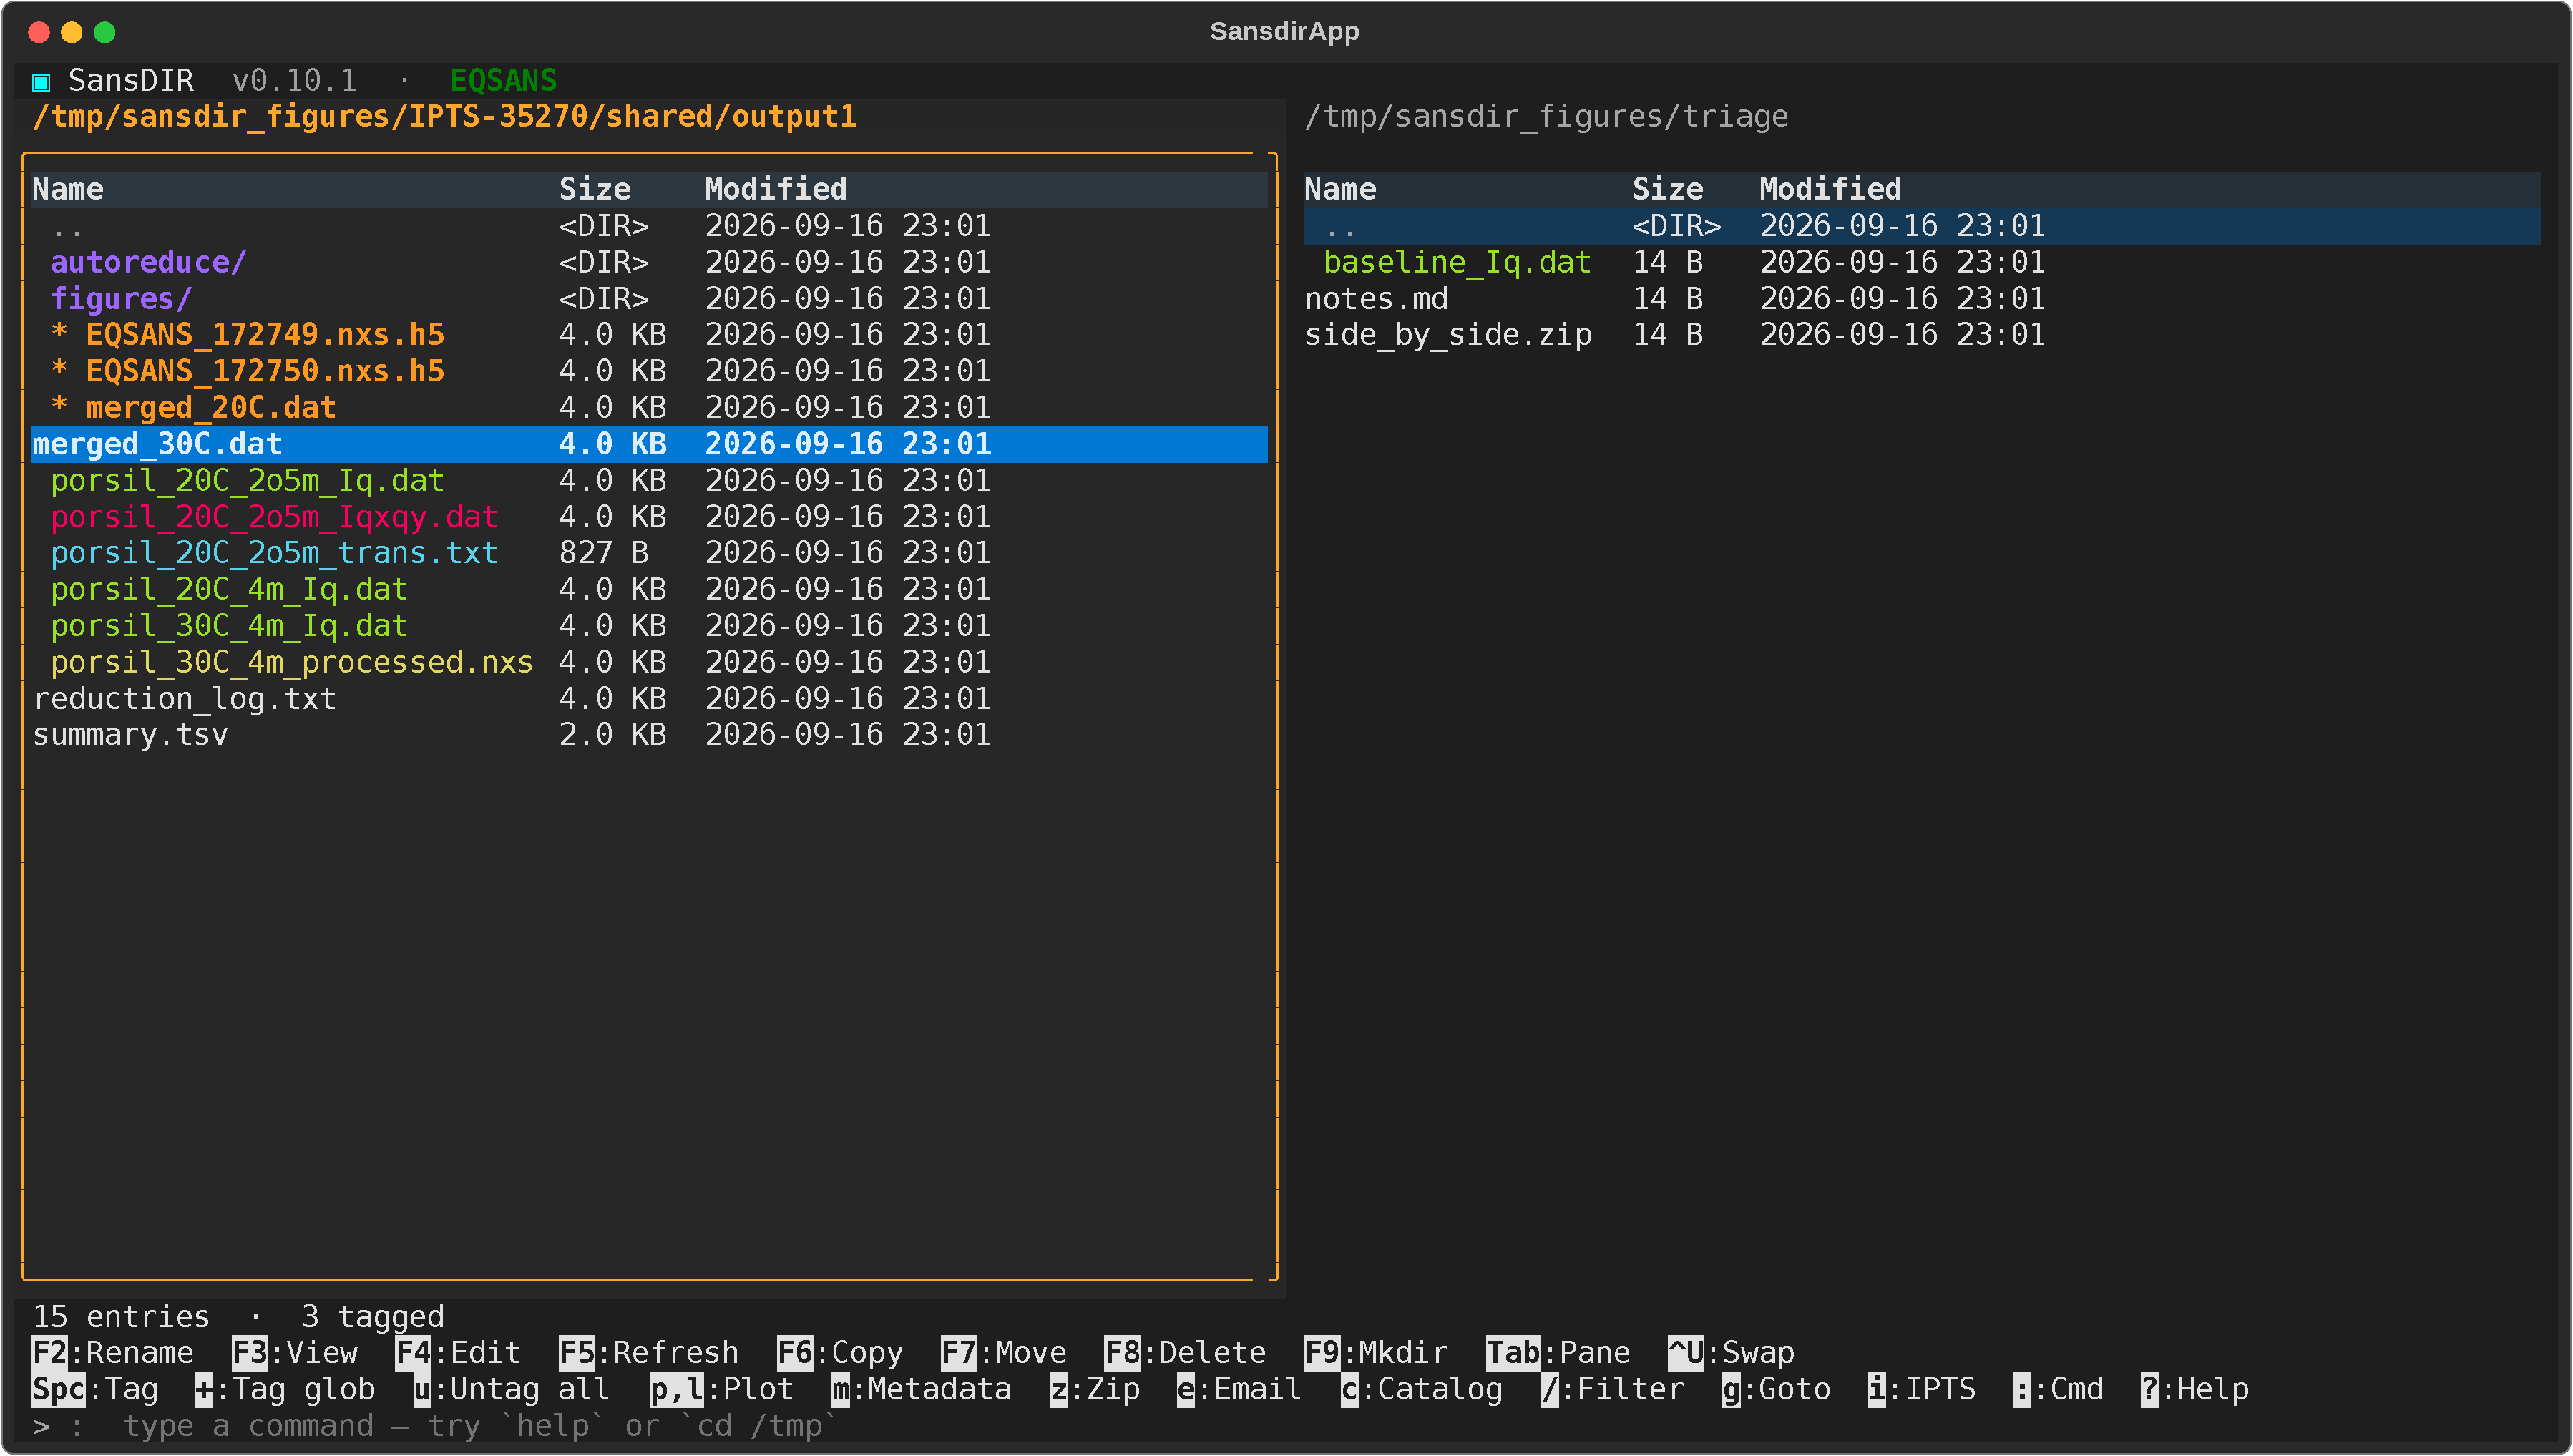
\includegraphics[width=\textwidth]{figures/tui-panes.pdf}
  \longcaption{The dual-pane interface.}{The left pane is active, indicated by
  the highlighted border and path. Three files are tagged, shown by the leading
  asterisk and the bold rendering; the status line reports the count. File kinds
  are distinguished by color: directories, one-dimensional reduced data,
  two-dimensional reduced data, transmission files, and NeXus files each have a
  distinct hue.}
  \label{fig:panes}
\end{figure}

The path bar rewrites the \texttt{/gpfs/neutronsfs/instruments} prefix to
\texttt{/SNS}, which is how the same location is conventionally written and how
users expect to see it, at no cost in accuracy since the two are the same mount.

\subsection{PANES AND ACTIVATION}

The two panes are instances of the same widget class holding independent state:
working directory, cursor position, tag set, sort key, and filter. Exactly one is
active at any moment, distinguished by border color. \key{Tab} switches
activation.

Several commands manipulate the pair rather than a single pane. \key{Ctrl+U}
swaps the two panes' contents, which is the fastest way to reverse the direction
of a copy. \key{=} synchronizes the inactive pane to the active pane's directory,
which is the usual preparation for a same-directory operation. \key{Ctrl+O}
maximizes the active pane to full width and restores it on a second press; this
is a toggle, never a default, because the dual-pane layout is the point.

The run catalog described in Section~\ref{sec:oncat} always occupies the right
pane regardless of which pane was active when it was requested. This keeps the
layout predictable: users learn that the catalog is on the right, and \key{Ctrl+U}
swaps file panes without disturbing it.

\subsection{FILE LISTING AND COLOR CODING}

Each pane lists name, size, and modification time. Directories sort first.
Sorting is by name, modification time, size, or extension, selected with the
number keys \key{1} through \key{4}. Hidden files are suppressed by default and
toggled with \key{h}. Symbolic links are followed but flagged.

Color encodes file kind so that a directory can be scanned at a glance
(Table~\ref{tab:colors}).

\begin{table}[ht]
  \centering
  \caption{File-kind color coding in the panes}
  \label{tab:colors}
  \small
  \begin{tabular}{l l}
    \toprule
    Kind & Rendering \\
    \midrule
    Directory & Bold blue \\
    Symbolic link & Cyan \\
    \texttt{*Iq*.dat}, one-dimensional reduced & Green \\
    \texttt{*Iqxqy*.dat}, two-dimensional reduced & Magenta \\
    \texttt{*trans*.txt}, transmission & Cyan \\
    \texttt{*.nxs.h5} and \texttt{*.nxs}, NeXus & Bright yellow \\
    Executable & Bold red \\
    Tagged row & Bold yellow with a leading asterisk \\
    \bottomrule
  \end{tabular}
\end{table}

\subsection{TAGGING}

Tagging is the selection mechanism for every multi-file operation.
\key{Space} toggles the tag on the row under the cursor. \key{+} prompts for a
glob and tags every visible entry matching it; \key{-} untags by glob; \key{u}
clears all tags in the active pane. Tags are per-pane and are cleared when that
pane changes directory.

The universal rule is that an operation acts on the active pane's tagged files
if there are any, and otherwise on the single file under the cursor. This means
the common single-file case requires no tagging at all, while the multi-file case
requires no separate ``select mode.''

\key{/} filters the active pane by substring, which composes naturally with
glob tagging: filter to a subset, tag everything visible, then act.

\subsection{COMMAND LINE AND HISTORY}

The command line is always visible at the bottom of the screen and is focused
with \key{:}. It accepts any registered command name or alias. Several keys are
shortcuts that pre-fill it rather than acting directly---\key{+} opens it
containing \texttt{tag.glob}, \key{g} containing \texttt{cd}, \key{F9}
containing \texttt{mkdir}---so that the relationship between a key and its
command is visible at the moment of use rather than only in the help overlay.

History persists across sessions in the cache directory.

\subsection{HELP OVERLAY}

\key{?} opens the help overlay of Figure~\ref{fig:help}. It is generated from the
registry and the key map at runtime. Because both are data, the overlay reflects
user key rebindings and cannot become inconsistent with the code.

%%%%%%%%%%%%%%%%%%%%%%%%%%%%%%%%%%%%%%%%%%%%%%%%%%%%%%%%%%%%%%%%%%%%%%%%%%%%%%%
% 5. NAVIGATION AND FILE OPERATIONS
%%%%%%%%%%%%%%%%%%%%%%%%%%%%%%%%%%%%%%%%%%%%%%%%%%%%%%%%%%%%%%%%%%%%%%%%%%%%%%%
\section{NAVIGATION AND FILE OPERATIONS}
\label{sec:fileops}

\subsection{NAVIGATION}

Table~\ref{tab:nav} lists the navigation keys. \key{Enter} is context-sensitive:
on a directory it descends, on an image it opens a viewer, and in the run catalog
it plots the run under the cursor.

\begin{table}[ht]
  \centering
  \caption{Navigation keys}
  \label{tab:nav}
  \small
  \begin{tabular}{l l}
    \toprule
    Key & Action \\
    \midrule
    \key{Tab} & Switch the active pane \\
    Arrow keys, \key{j} \key{k} & Move the cursor \\
    \key{Enter} & Descend into a directory, open an image, or plot a catalog
      row \\
    \key{Backspace} & Ascend one directory \\
    \key{g} & Prompt for a path \\
    \key{G} & Full-screen directory-tree browser \\
    \key{/} & Filter the active pane by substring \\
    \key{=} & Synchronize the inactive pane to the active pane's directory \\
    \key{Ctrl+U} & Swap the two panes \\
    \key{Ctrl+O} & Maximize or restore the active pane \\
    \bottomrule
  \end{tabular}
\end{table}

\subsection{FILE OPERATION SEMANTICS}

File operations follow the Norton Commander convention: they act on the active
pane's selection, and the default destination is the \emph{inactive} pane's
working directory. Table~\ref{tab:fkeys} lists the function-key assignments.

\begin{table}[ht]
  \centering
  \begin{threeparttable}
  \caption{Function-key file operations}
  \label{tab:fkeys}
  \small
  \begin{tabular}{l l p{0.52\textwidth}}
    \toprule
    Key & Operation & Behavior \\
    \midrule
    \key{F2} & Rename & In-place rename of the file under the cursor. \\
    \key{F3} & View & Read-only view in the opposite pane; \key{Esc} or a
      second \key{F3} closes it. \\
    \key{F4} & Edit & Opens \texttt{\$EDITOR}. \\
    \key{F5} & Refresh & Re-reads both directory listings. \\
    \key{F6} & Copy & Selection into the inactive pane, after confirmation. \\
    \key{F7} & Move & As copy, then removes the source. \\
    \key{F8} & Delete & Always confirms; uses \texttt{send2trash} where
      available. \\
    \key{F9} & Make directory & Prompts in the active pane. \\
    \key{c} & Catalog toggle & Flips the inactive pane between file list and run
      catalog.\tnote{a} \\
    \bottomrule
  \end{tabular}
  \begin{tablenotes}
    \item[a] The catalog toggle is bound to \key{c} rather than \key{F10}
    because most terminal emulators intercept \key{F10} for their own menu bar.
    The classic copy, move, and delete bindings are correspondingly shifted from
    \key{F5}--\key{F7} to \key{F6}--\key{F8} to make room for refresh.
  \end{tablenotes}
  \end{threeparttable}
\end{table}

Two behaviors deserve specific mention because they were adopted after user
feedback. First, after a delete the cursor remains adjacent to the deleted
entry---on the row that took its place, or on the new last row if the deleted
file was last---rather than jumping to the top of the list. Cleaning up several
files individually is otherwise punishing. Second, all destructive operations
confirm before acting, and all are logged.

\subsection{REFRESH BEHAVIOR}

Operations performed inside the application---copy, move, rename, make
directory, batch extract, archive creation---refresh the affected panes
automatically. \key{F5} is the manual fallback for changes made by an external
agent: a second shell session writing into a pane's directory, an autoreduction
job depositing new output, or \ac{nfs} attribute caching catching up.

The mask editor is a hybrid case. It runs as a detached subprocess so the
interface stays responsive, but its launcher awaits the exit code in a worker;
an exit indicating a save triggers a refresh of both panes so the new mask file
appears without user action.

\subsection{ARCHIVING AND EMAIL}

\key{z} creates a zip archive of the selection, prompting for the archive name
and defaulting to the inactive pane's directory. A gzip-compressed tar
alternative is available as \cmd{archive.tar\_gz} on the command line. \key{e}
opens a dialog that sends the selection as attachments by shelling out to
\texttt{mail} or \texttt{mutt}, whichever is configured.

\subsection{SHELL ESCAPE}

\cmd{shell.run}, aliased to \texttt{!}, runs an arbitrary shell command with the
interface suspended, restoring it when the command exits. This is the escape
hatch for the operations the program does not implement.

%%%%%%%%%%%%%%%%%%%%%%%%%%%%%%%%%%%%%%%%%%%%%%%%%%%%%%%%%%%%%%%%%%%%%%%%%%%%%%%
% 6. PLOTTING
%%%%%%%%%%%%%%%%%%%%%%%%%%%%%%%%%%%%%%%%%%%%%%%%%%%%%%%%%%%%%%%%%%%%%%%%%%%%%%%
\section{PLOTTING}
\label{sec:plot}

\subsection{PLOTTING THE SELECTION}

Plotting is invoked with a single key, \key{p}, on the active selection: the
tagged files if there are any, otherwise the file under the cursor. The program
decides what to draw from the file itself rather than asking, so the same
keystroke serves every kind of \ac{sans} data. Table~\ref{tab:plotrouting}
summarizes what each kind produces.

\begin{table}[ht]
  \centering
  \caption{What \key{p} draws for each kind of file}
  \label{tab:plotrouting}
  \small
  \begin{tabular}{p{0.30\textwidth} p{0.60\textwidth}}
    \toprule
    Selection & Result \\
    \midrule
    \texttt{*Iq*.dat}, 2--4 columns & Logarithmic $I(q)$ plot, with error bars
      when a $\sigma_I$ column is present. Several files overlay on shared
      axes. \\
    \texttt{*trans*.txt} & Transmission $T(\lambda)$ on linear axes,
      $\lambda$ in \AA. \\
    \texttt{*Iqxqy*.dat}, 4 or 6 columns & Two-dimensional heat map; several
      files tile into one window. \\
    \texttt{*.nxs.h5} raw event file & Detector heat map of summed counts. \\
    \texttt{*.nxs} processed Mantid file & Detector heat map through the same
      view. \\
    Any other tabular file (\key{l}) & Linear plot using the header row as axis
      labels. \\
    \bottomrule
  \end{tabular}
\end{table}

Plots open in their own windows, so the terminal stays usable while a figure is
on screen and several figures can be open at once. On a host with no display
the figure is instead written as a \ac{png} under
\texttt{\hme/.cache/sansdir/plots/} and the path is reported in the status bar,
so the same keystroke works over a plain \ac{ssh} session with no forwarding.

Classification does not rely on the file extension alone, which matters because
Mantid writes processed output as \texttt{.nxs} without the \texttt{.h5} suffix
and reduced files are not always named predictably. A file whose contents are
\ac{hdf} is treated as NeXus whatever it is called, and column count and header
keywords disambiguate the ASCII kinds.

\subsection{ONE-DIMENSIONAL PLOTS}

Reduced $I(q)$ files are drawn on logarithmic axes by default, with error bars
when a third column is present. Tagging several files overlays them on shared
axes with a filename legend, which is the common comparison case: the same sample
at two temperatures, or the same measurement at two detector distances.
Figure~\ref{fig:iq} shows a representative single-curve plot.

\begin{figure}[ht]
  \centering
  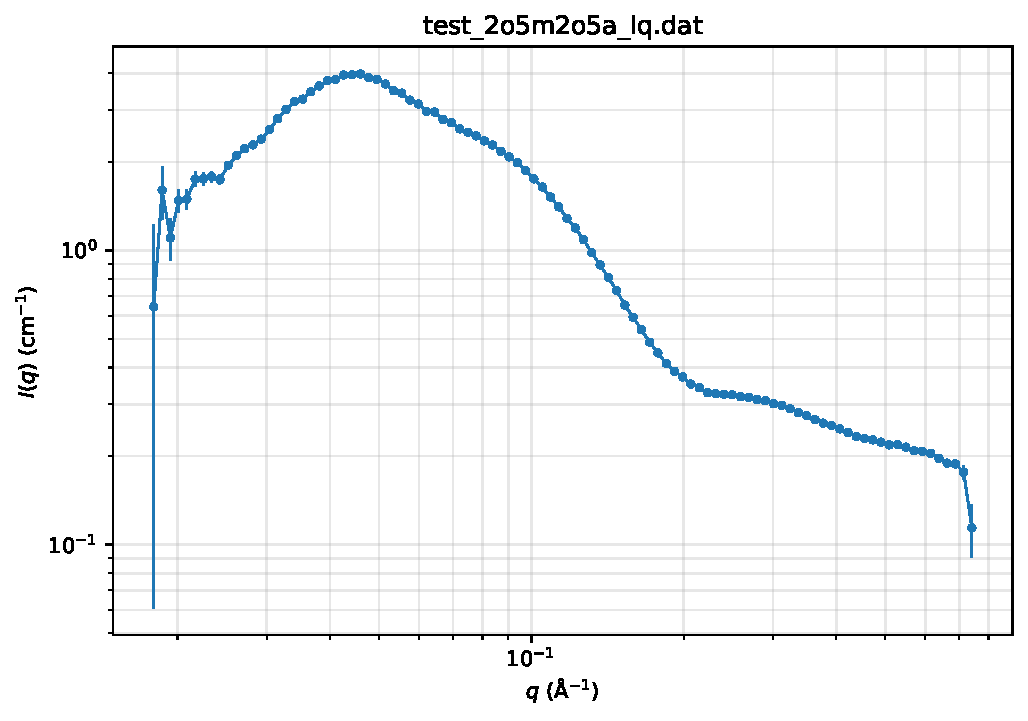
\includegraphics[width=0.78\textwidth]{figures/plot-iq.pdf}
  \longcaption{One-dimensional reduced data.}{A three-column $I(q)$ file plotted
  on logarithmic axes with error bars. Axis labels and units are applied
  automatically. This figure was produced by the same code path the \key{p} key
  invokes.}
  \label{fig:iq}
\end{figure}

Transmission files are treated differently: linear axes, wavelength in \AA{} on
the abscissa, and transmission on the ordinate, with labels and title to match.

\subsection{TWO-DIMENSIONAL PLOTS}

Four- and six-column $I(q_x,q_y)$ files are drawn as a heat map on proper $q_x$
and $q_y$ axes. A logarithmic color scale is the default, which for scattering
data is almost always what is wanted.

Tagging more than one two-dimensional file tiles them into a single window with
the filename as each subplot title. Two color bar modes are available: shared,
using common limits across all panels so that intensities are directly
comparable, and independent, using per-panel limits so that weak patterns
remain visible.

\subsection{DETECTOR HEAT MAPS FROM NEXUS}

Raw EQ-SANS \autocite{eqsans} event files are rendered as a
$256\times192$ detector image, as shown in Figure~\ref{fig:detector}. Processed
Mantid files---including wavelength-banded \texttt{drtsans} output and
event-workspace masks---render through the same view.

\begin{figure}[ht]
  \centering
  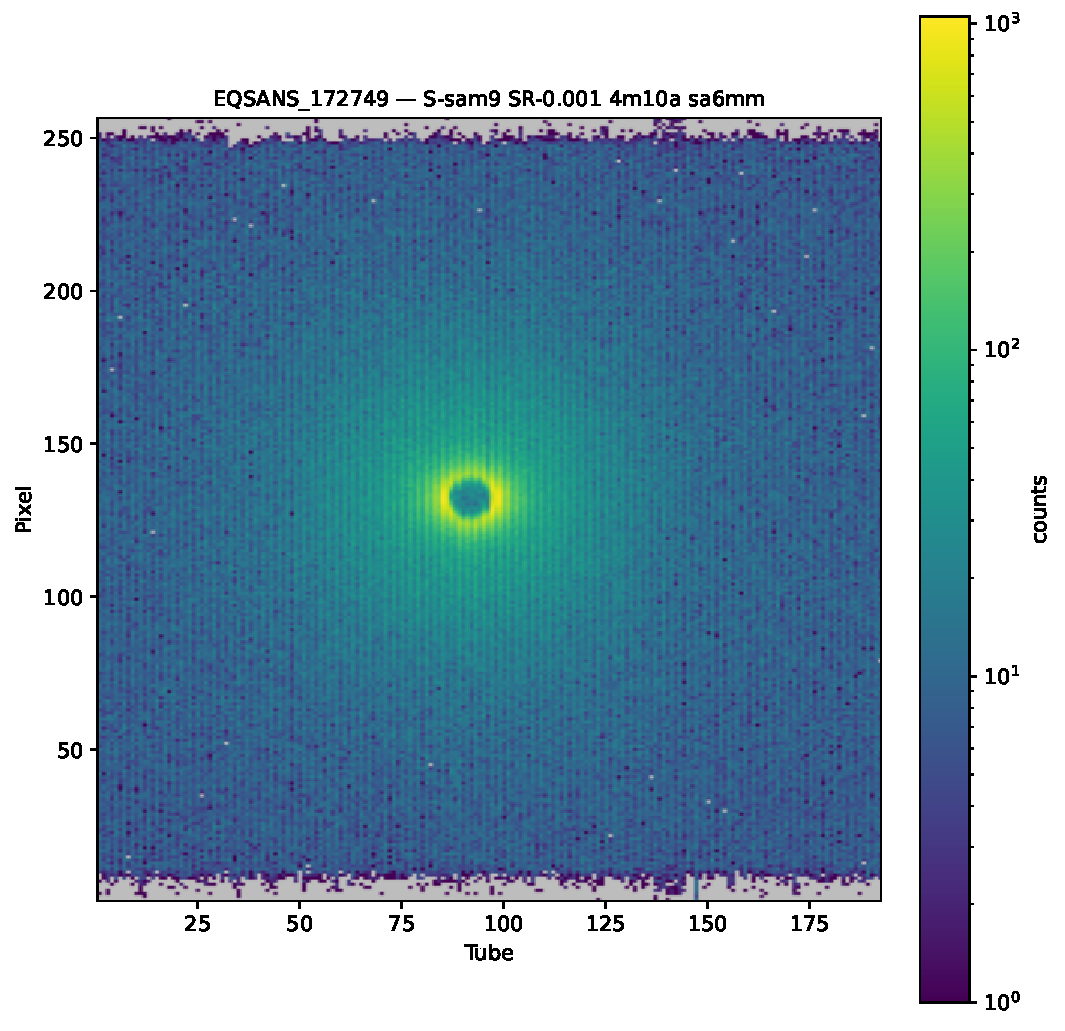
\includegraphics[width=0.72\textwidth]{figures/plot-detector.pdf}
  \longcaption{Detector heat map from a raw NeXus event file.}{Counts summed over
  all events and reordered into the physical tube-and-pixel layout, on a
  logarithmic color scale. The beam stop is visible at the center of the direct
  beam. The reconstruction is performed entirely in \texttt{numpy}; no Mantid
  runtime is involved.}
  \label{fig:detector}
\end{figure}

The image is reconstructed from the event arrays without invoking Mantid, so the
detector view stays available on hosts where no Mantid environment is installed
or where one is mid-upgrade.

\subsection{GENERIC TABULAR PLOTS}

\key{l} plots any whitespace-, comma-, or tab-delimited table on linear axes,
taking axis labels from the header row. This is the companion to the batch
metadata extractor of Section~\ref{sec:meta}: extract temperature against time
across a series of runs, then plot the resulting table without leaving the
program.

Static images---\ac{png}, JPEG, TIFF, and similar---open in a matplotlib window
on \key{Enter}, which is convenient for the figures deposited by autoreduction.

%%%%%%%%%%%%%%%%%%%%%%%%%%%%%%%%%%%%%%%%%%%%%%%%%%%%%%%%%%%%%%%%%%%%%%%%%%%%%%%
% 7. METADATA
%%%%%%%%%%%%%%%%%%%%%%%%%%%%%%%%%%%%%%%%%%%%%%%%%%%%%%%%%%%%%%%%%%%%%%%%%%%%%%%
\section{METADATA INSPECTION AND EXTRACTION}
\label{sec:meta}

\subsection{SINGLE-FILE TREE BROWSER}

\key{m} opens the file under the cursor in a modal tree browser. The hierarchy
expands lazily: only the direct children of an expanded group are read. This is
necessary rather than merely efficient---an exhaustive walk of a
several-hundred-megabyte raw file yields tens of thousands of entries and takes
seconds, which is both slow and unreadable.

Selecting a leaf displays its full path, dtype, shape, units taken from the
\texttt{units} attribute, and a one-line value preview.

\subsection{KEYWORD SEARCH}
\label{sec:hdfsearch}

Lazy expansion solves the loading problem but creates a navigation one. Sample
environment logs live at paths such as
\texttt{/entry/DASlogs/BL6:SE:QNTC1:ReadProbeTemperature/value}, and reaching one
by expanding groups requires knowing the instrument's device naming scheme.

Pressing \key{/} in the tree browser therefore switches to keyword search. The
full key list is walked once, on a worker thread, and cached; subsequent queries
filter it by case-insensitive substring. Results are shown as a table of matching
paths with their shapes, and the detail pane follows the highlighted row, so
\key{Up} and \key{Down} scan candidates without leaving the search box.
Figure~\ref{fig:hdfsearch} shows the result of searching a real EQ-SANS file for
\texttt{temperature}: 28 matches across three distinct devices, located without
any knowledge of the naming convention.

\begin{figure}[ht]
  \centering
  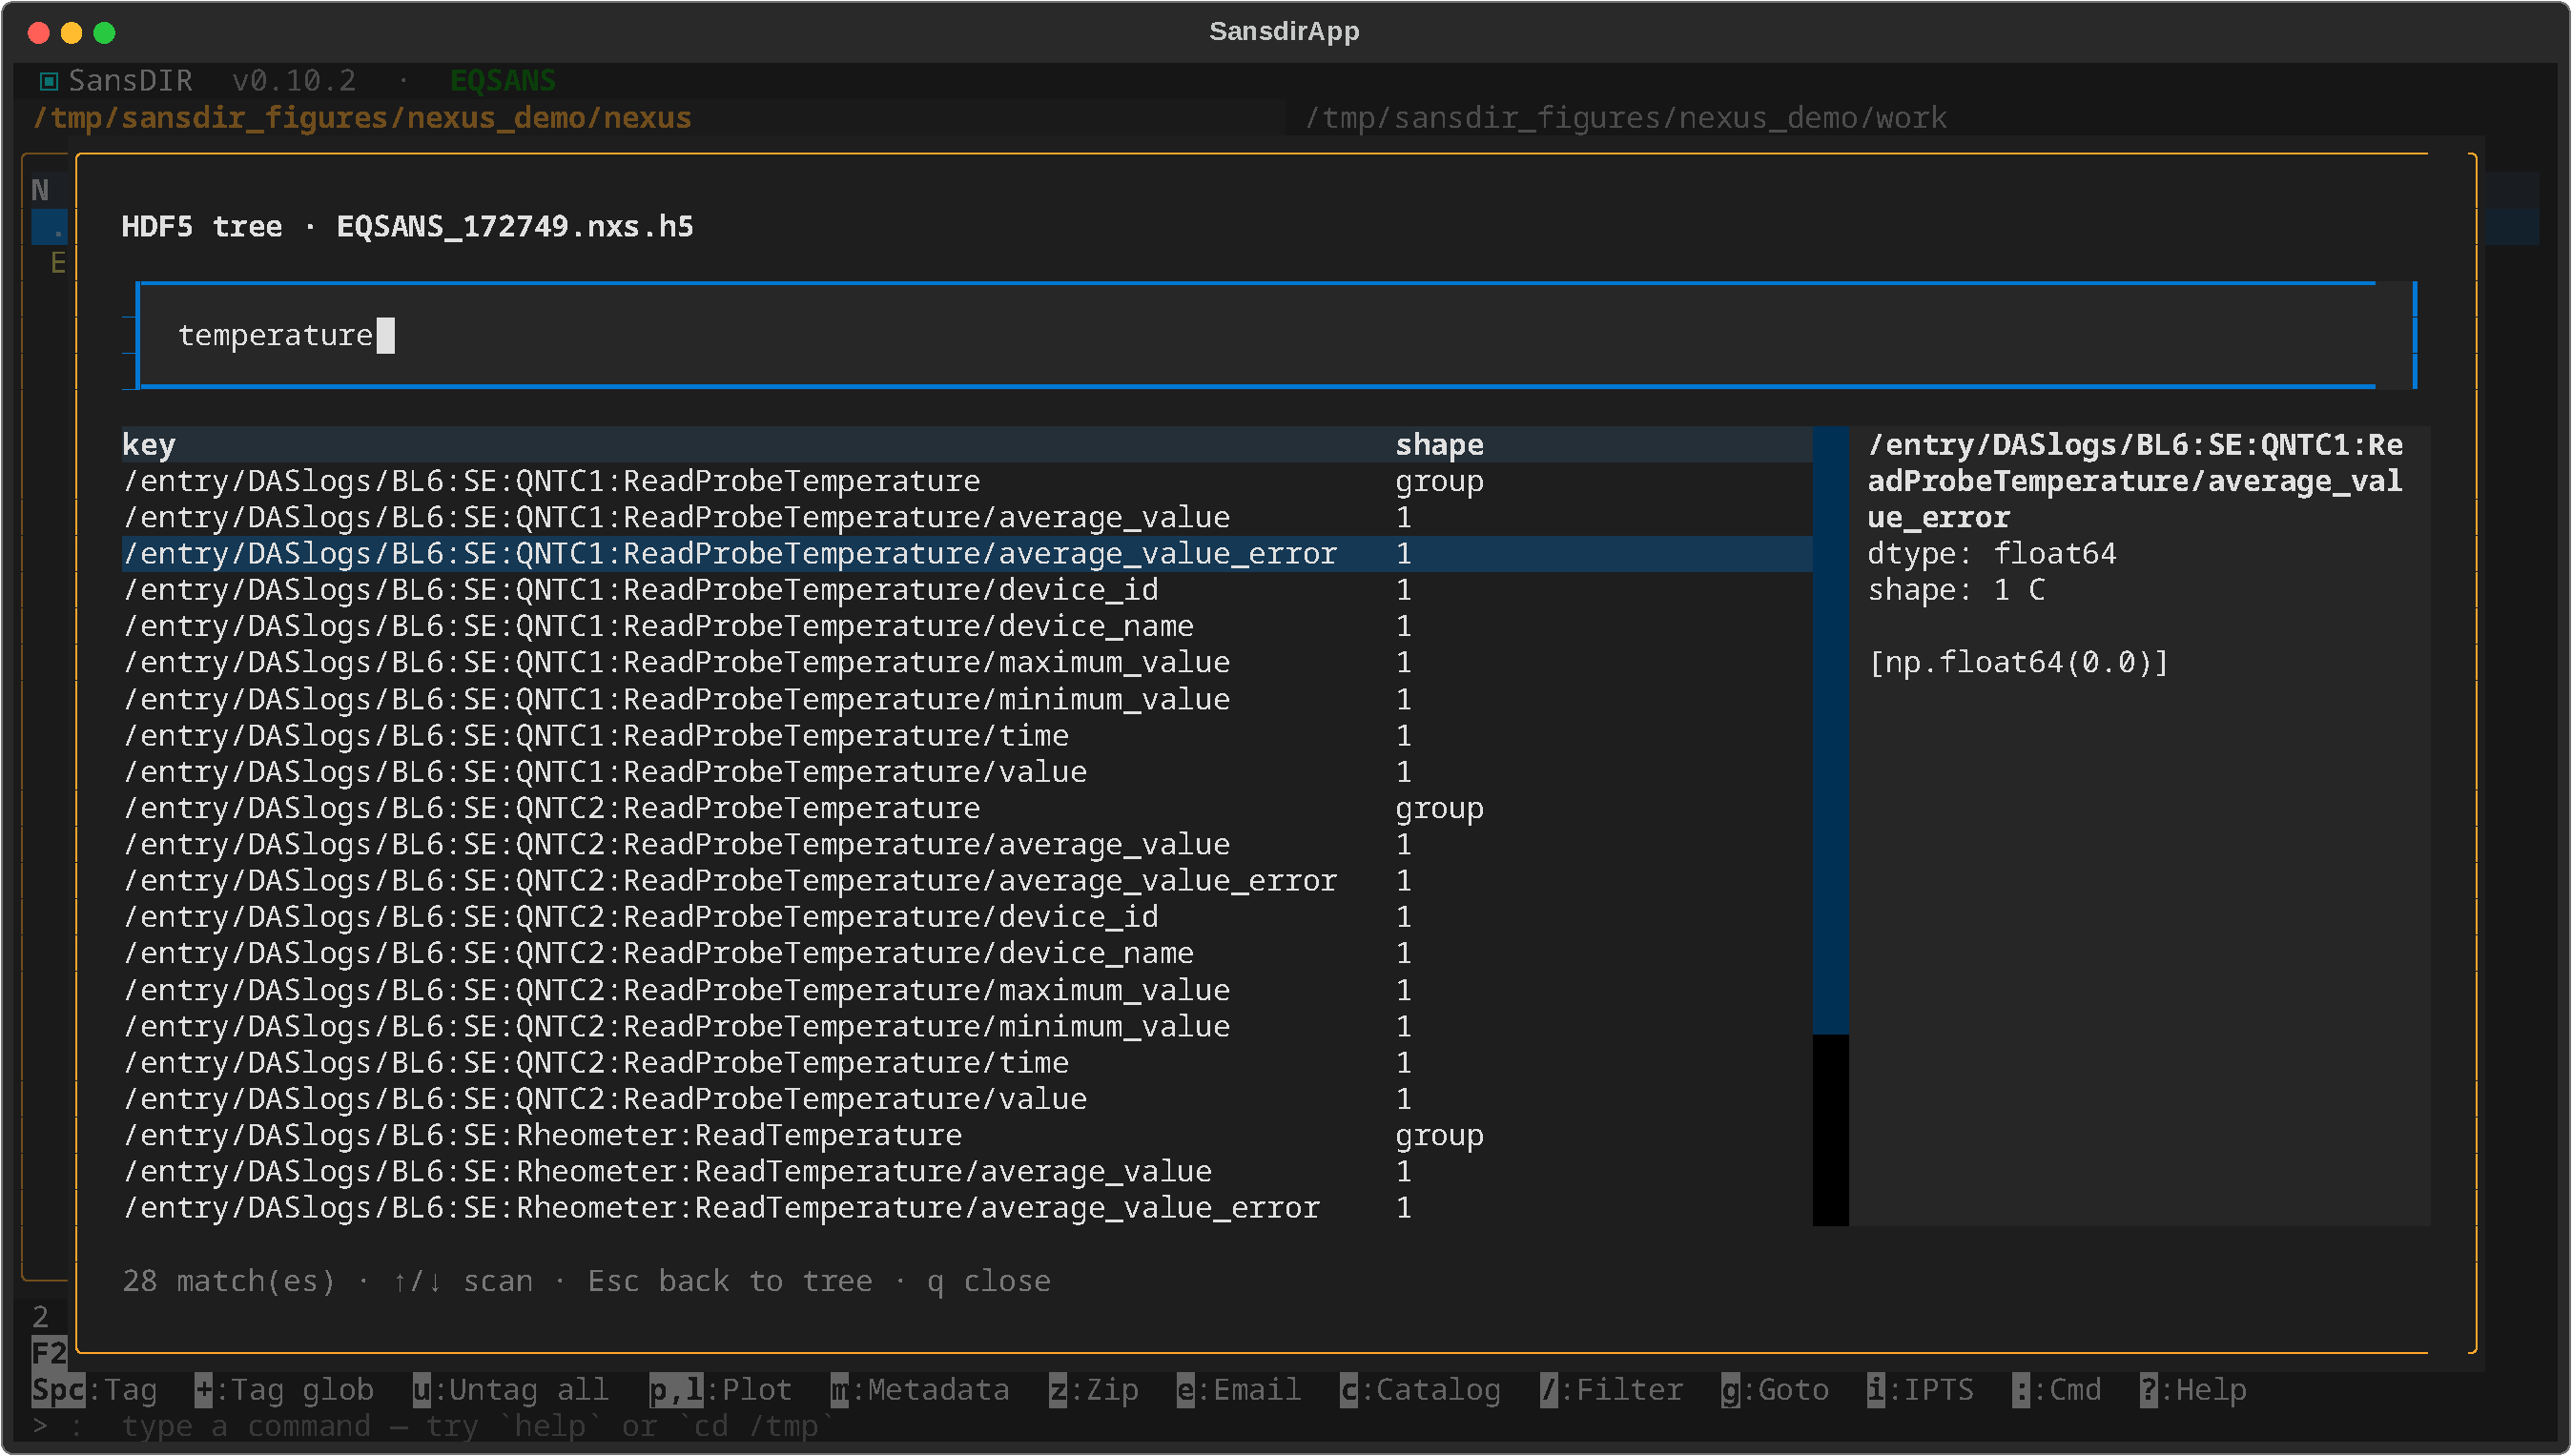
\includegraphics[width=\textwidth]{figures/hdf-search.pdf}
  % Literal "HDF5" rather than \ac{hdf}: the first argument becomes the
  % List of Figures entry, where acro's counter is fresh and would expand to
  % the long form.
  \longcaption{Keyword search in the HDF5 tree browser.}{A substring query
  against a raw EQ-SANS file. The left table lists matching keys with their
  shapes; the right pane shows the highlighted key's dtype, shape, and value
  preview. \key{Esc} returns to the tree view, and a second \key{Esc} closes the
  browser.}
  \label{fig:hdfsearch}
\end{figure}

Two bounds keep the feature responsive on large files. Rendered matches are
capped at 500, with the hint line stating explicitly when a query was truncated
rather than silently discarding the remainder. Value previews slice before
materializing, so previewing a multi-million-element event array reads five
values rather than the whole array.

\subsection{BATCH EXTRACTION}

\key{M} extracts selected keys from many files at once. The dialog opens with a
full-screen key picker in which \key{Space} toggles a key and \key{/} searches
across all keys in the file, using the same search mechanism as the single-file
browser. \key{Ctrl+S} returns to the output form.

Extraction is parallel: \texttt{h5py} releases the interpreter lock during reads,
so a thread pool---eight workers by default---scales nearly linearly with file
count.

The key picker accepts a group as well as a dataset when the group contains a
\texttt{value} child, which is the \ac{sns} \ac{das} log convention. Selecting the
group is equivalent to selecting \texttt{<group>/value}, which is what the user
means.

\subsection{OUTPUT MODES}

Two output modes cover the two distinct questions users ask.

\textbf{Summary mode} produces one row per input file, with time-series values
reduced to their mean. This answers ``what was the temperature for each of these
40 runs.'' Optional \texttt{\_stdev} and \texttt{\_n} columns report the spread
and sample count behind each mean.

\textbf{Per-file mode} produces one table per input file with the full arrays
preserved. This answers ``how did temperature evolve during this run.'' It is
selected by including the placeholder \texttt{<filename>} in the output template,
for example \texttt{<filename>\_temp.csv}. If the user requests per-file mode but
omits the placeholder, the program prepends \texttt{<filename>\_} rather than
overwriting one file repeatedly.

Output is written to the inactive pane's working directory by default, because
the active pane is typically the read-only proposal directory and defaulting
there would produce a permission error on every attempt.

%%%%%%%%%%%%%%%%%%%%%%%%%%%%%%%%%%%%%%%%%%%%%%%%%%%%%%%%%%%%%%%%%%%%%%%%%%%%%%%
% 8. ONCAT
%%%%%%%%%%%%%%%%%%%%%%%%%%%%%%%%%%%%%%%%%%%%%%%%%%%%%%%%%%%%%%%%%%%%%%%%%%%%%%%
\section{CATALOG INTEGRATION}
\label{sec:oncat}

\subsection{AUTHENTICATION}

OnCat requires an \ac{oauth} bearer token even for read-only endpoints. The
client obtains one through the client-credentials grant and caches it until
shortly before expiry. Credentials come from the \texttt{[oncat]} configuration
section or from the \texttt{ONCAT\_CLIENT\_ID} and \texttt{ONCAT\_CLIENT\_SECRET}
environment variables, with working defaults so that a cluster user gets a
functioning search without configuration. The endpoint is likewise configurable,
so the client can be pointed at a staging instance.

\subsection{SEARCH MODEL AND CACHING}

OnCat exposes no fuzzy keyword endpoint. The client therefore lists all
experiments for the configured instrument once, caches the listing on disk for a
configurable \ac{ttl} defaulting to 24~hours, and filters client-side on
substring matches against the proposal identifier, the title, and the member
list. The first search pays one server round trip; every subsequent search is
served from cache and completes in well under a second.

Because a stale cache can hide a newly allocated proposal, \key{r} in the browser
forces a cache-bypassing refetch.

The browser keeps typing responsive on large catalogs in two ways. The filter
input is debounced with a 200~ms quiet window, so a fast typist causes one
rebuild rather than one per keystroke. The rendered result set is capped at 200
rows, with an overflow hint reporting how many further matches exist.

\subsection{RUN CATALOG PANE}

Selecting a proposal changes the active pane into that proposal's
\texttt{shared/} directory and loads its run list into a catalog view on the
right pane. \key{c} toggles the catalog. Within it, \key{Space} tags runs and the
familiar keys operate on the selection: \key{Enter} or \key{p} plots the raw
detector image, \key{m} opens the \ac{hdf} tree, \key{M} extracts metadata, and
\key{K} opens the mask editor. The catalog is thus a third selection surface
sharing the same command vocabulary as the two file panes.

%%%%%%%%%%%%%%%%%%%%%%%%%%%%%%%%%%%%%%%%%%%%%%%%%%%%%%%%%%%%%%%%%%%%%%%%%%%%%%%
% 9. MASK
%%%%%%%%%%%%%%%%%%%%%%%%%%%%%%%%%%%%%%%%%%%%%%%%%%%%%%%%%%%%%%%%%%%%%%%%%%%%%%%
\section{DETECTOR MASK CREATION}
\label{sec:mask}

\subsection{ARCHITECTURAL CONSTRAINTS}

Detector masking is the one feature that produces an input to reduction rather
than a view of its output. Three constraints bound the implementation:

\begin{itemize}
  \item \textbf{No Mantid runtime imports in the package.} Searching the source
    tree for Mantid imports returns nothing. Mask \emph{creation} is pure Python.
    A Mantid environment is invoked only as an external subprocess, and only at
    save time, as described below.
  \item \textbf{No instrument-specific geometry in the source.} There is no
    per-instrument pixel-to-detector formula. The detector mapping is recovered
    from the source NeXus file itself, from its event-identifier-to-detector
    correspondence.
  \item \textbf{Pixel ordering is defined in exactly one place.} The invariant
    that the flattened mask array aligns element-for-element with the pixel
    identifier array is established in a single module, and the writers consume
    that invariant rather than re-deriving it.
\end{itemize}

The masking convention follows Mantid: 1 denotes a masked, excluded pixel and 0 a
kept one, so that passing the output to \texttt{MaskDetectors} excludes exactly
the cells the user drew. Inverting the final mask is a single flag.

\subsection{INTERACTIVE EDITOR}

\key{K}, from a file pane or the run catalog, opens a matplotlib window showing
the detector heat map of the selected file. The user draws shapes on it.

The cell aspect ratio is set to $1/1.3$ to compensate for the EQ-SANS detector's
tube pitch of roughly 5.2~mm against a pixel pitch of roughly 3.9~mm. Without
this correction an ellipse drawn to look circular on screen is not circular on
the detector. The canvas extends a few cells beyond the detector boundary, which
is marked with a faint dotted line, so that a rubber-band selection can be
dragged from outside the active area---otherwise masking the outermost row
requires landing the first click exactly on pixel zero.

Table~\ref{tab:maskkeys} lists the editor's controls.

\begin{table}[ht]
  \centering
  \caption{Interactive mask editor controls}
  \label{tab:maskkeys}
  \small
  \begin{tabular}{l p{0.72\textwidth}}
    \toprule
    Key & Action \\
    \midrule
    \key{r} & Rectangle draw mode \\
    \key{e} & Ellipse draw mode \\
    \key{v} & Edit mode: click to select a shape, drag to move it, \key{Delete}
      to remove it \\
    \key{k} & Open the bank and tube specification dialog \\
    \key{z} & Undo \\
    \key{i} & Invert the mask \\
    \key{s} & Save, through a file chooser \\
    \key{Esc} & Quit without saving \\
    \bottomrule
  \end{tabular}
\end{table}

The bank and tube dialog accepts a compact specification language---\texttt{b3}
for a whole bank, \texttt{t50} for a tube, \texttt{b5-7 t10-15} for mixed
ranges---which covers the strip-masking case far better than freehand drawing.
The resulting rectangles are ordinary shapes and round-trip through the mask log
like any other.

Two responsiveness measures are worth recording because both replaced an
implementation that was correct but unusable. Moving a shape in edit mode
snapshots the static canvas on mouse-down and re-blits only the moving patch on
each motion event, rather than redrawing the full heat map. And the bank and tube
input is a dialog rather than an inline matplotlib text widget, because that
widget redraws on every keystroke, which on a logarithmically scaled
$256\times192$ image is visible per-character lag.

A cursor readout reports \texttt{tube}, \texttt{pixel}, \texttt{counts},
\texttt{bank}, and the tube index within its bank as the pointer moves, which is
what allows a user to translate a visual feature into a bank and tube
specification.

\subsection{COMMAND-LINE MASK CREATION}

The same functionality is available non-interactively. Shapes are given in pixel
coordinates and the options are repeatable:

\begin{lstlisting}[language=shellsession]
sansdir mask /SNS/EQSANS/IPTS-XXXXX/nexus/EQSANS_172749.nxs.h5 \
  --circle 96,128,12 \
  --rect 0,0,15,15   --rect 176,0,191,15 \
  --rect 0,240,15,255 --rect 176,240,191,255 \
  --output beam_stop.nxs
\end{lstlisting}

Available shapes are \texttt{--rect X0,Y0,X1,Y1}, \texttt{--ellipse
XC,YC,RX,RY}, \texttt{--circle XC,YC,R}, and \texttt{--polygon
X1,Y1,X2,Y2,...} with at least three vertices. A sidecar log in \ac{json} form
is written alongside every output, and \texttt{--shapes-json} replays it, so a
mask developed interactively can be reapplied to other runs in a script.

\subsection{OUTPUT FORMATS AND REDUCTION COMPATIBILITY}

Three output formats are supported: a Mantid \texttt{SaveMask} \ac{xml} file, a
NeXus file, and a \texttt{numpy} array with a metadata sidecar.

The NeXus path deserves explanation because it changed during development. To be
usable by the \texttt{drtsans} reduction pipeline, the mask must carry per-detector
mask flags in the instrument parameter map that the pipeline reads. Producing
that structure reliably means letting Mantid write it. The save step therefore
shells out to the cluster's \texttt{drtsans} wrapper to run a
load--mask--save sequence against the source file. When Mantid is unavailable,
the program falls back to a pure-\texttt{numpy} writer that produces a
visualization-only file, and says so: the fallback output can be inspected but
does not affect reduction.

The on-disk encoding of the visualization file mirrors the convention of existing
EQ-SANS beam-stop files, in which each \emph{unmasked} detector carries one
synthetic event and masked detectors carry none. Consequently a mask opened with
\key{p} renders with the masked region in grey, the same visual convention as a
beam stop. The builder retains Mantid's ``1 means masked'' convention internally;
only the on-disk encoding is inverted.

%%%%%%%%%%%%%%%%%%%%%%%%%%%%%%%%%%%%%%%%%%%%%%%%%%%%%%%%%%%%%%%%%%%%%%%%%%%%%%%
% 10. CLI
%%%%%%%%%%%%%%%%%%%%%%%%%%%%%%%%%%%%%%%%%%%%%%%%%%%%%%%%%%%%%%%%%%%%%%%%%%%%%%%
\section{NON-INTERACTIVE COMMAND-LINE INTERFACE}
\label{sec:cli}

Three operations are available without the \ac{tui}, for use in scripts and
batch jobs. Because they dispatch through the same registry, their behavior
matches the interactive equivalents exactly.

\subsection{LAUNCHING THE INTERFACE}

\begin{lstlisting}[language=shellsession]
sansdir                                # TUI in the current directory
sansdir /SNS/EQSANS/IPTS-12345/shared  # TUI rooted at a directory
\end{lstlisting}

A bare path argument is interpreted as \texttt{sansdir tui PATH}, so the
subcommand name may be omitted in the common case.

\subsection{BATCH METADATA EXTRACTION}

\begin{lstlisting}[language=shellsession]
# Summary table: one row per file, time series reduced to means.
sansdir extract \
  -k /entry/DASlogs/temperature/value \
  -k /entry/duration \
  --out summary.tsv \
  /SNS/EQSANS/IPTS-12345/nexus/EQSANS_*.nxs.h5

# Per-file tables: each input gets its own CSV with full arrays.
sansdir extract \
  -k /entry/DASlogs/temperature/time \
  -k /entry/DASlogs/temperature/value \
  --out '<filename>_temp.csv' \
  EQSANS_172749.nxs.h5 EQSANS_172750.nxs.h5

# Add spread and sample-count columns (summary mode only).
sansdir extract --with-stats -k /entry/DASlogs/temperature/value *.nxs.h5
\end{lstlisting}

Options are \texttt{-k/--keys} (repeatable, required), \texttt{-o/--out},
\texttt{--format} with values \texttt{tsv}, \texttt{csv}, or \texttt{columns},
\texttt{--with-stats}, and \texttt{--workers} to size the thread pool. The
written paths are echoed to standard output, one per line, so the command
composes with shell pipelines.

\subsection{MASK CREATION}

The \texttt{mask} subcommand is documented in Section~\ref{sec:mask}. Its options
are \texttt{--rect}, \texttt{--ellipse}, \texttt{--circle}, \texttt{--polygon},
\texttt{--shapes-json}, \texttt{--inverse}, \texttt{--output}, and
\texttt{--format} with values \texttt{nxs}, \texttt{xml}, or \texttt{npy}. On
completion it reports the output path, the masked pixel count as an absolute
number and a percentage, and the sidecar log path.

%%%%%%%%%%%%%%%%%%%%%%%%%%%%%%%%%%%%%%%%%%%%%%%%%%%%%%%%%%%%%%%%%%%%%%%%%%%%%%%
% 11. CONFIGURATION
%%%%%%%%%%%%%%%%%%%%%%%%%%%%%%%%%%%%%%%%%%%%%%%%%%%%%%%%%%%%%%%%%%%%%%%%%%%%%%%
\section{CONFIGURATION}
\label{sec:config}

Configuration is read from \texttt{\hme/.config/sansdir/config.toml}, or from the
path named by \texttt{\$SANSDIR\_CONFIG}. Every section and key is optional; the
program runs correctly with no configuration file at all.

\begin{lstlisting}
[ui]
theme = "monokai"       # any Textual theme name

[keys]
"ctrl+y" = "view.toggle_hidden"   # rebind any key to any command
f5 = "ui.move_tagged"             # unknown commands are dropped at startup

[oncat]
default_instrument = "EQSANS"
cache_ttl_seconds  = 86400

[mail]
command = "mail"                  # or "mutt"
default_subject = "[sansdir] data"
\end{lstlisting}

The loader is deliberately tolerant. An unknown theme name falls back to the
default with a notification rather than aborting startup, and a key rebinding
naming a nonexistent command is dropped with a notification. A malformed
configuration file should never prevent the program from launching, because a
user who cannot launch the program also cannot use it to fix the file.

Themes may also be changed at runtime with \texttt{:theme <name>}; issuing
\texttt{:theme} with no argument lists the available names.

%%%%%%%%%%%%%%%%%%%%%%%%%%%%%%%%%%%%%%%%%%%%%%%%%%%%%%%%%%%%%%%%%%%%%%%%%%%%%%%
% 12. DATA FORMATS
%%%%%%%%%%%%%%%%%%%%%%%%%%%%%%%%%%%%%%%%%%%%%%%%%%%%%%%%%%%%%%%%%%%%%%%%%%%%%%%
\section{SUPPORTED DATA FORMATS}
\label{sec:formats}

\subsection{ASCII REDUCED DATA}

Reduced data files are whitespace-delimited ASCII with optional comment lines
introduced by \texttt{\#}. Table~\ref{tab:formats} gives the recognized column
layouts. Detection counts the columns on the first non-comment line.

\begin{table}[ht]
  \centering
  \begin{threeparttable}
  \caption{Recognized ASCII column layouts}
  \label{tab:formats}
  \small
  \begin{tabular}{l c l p{0.34\textwidth}}
    \toprule
    Kind & Columns & Layout & Treatment \\
    \midrule
    \multirow{3}{*}{$I(q)$}
      & 2 & $q$, $I(q)$ & Logarithmic axes \\
      & 3 & $q$, $I(q)$, $\sigma_I$ & Logarithmic axes with error bars \\
      & 4 & $q$, $I(q)$, $\sigma_I$, $\sigma_q$ & As three-column; the
        resolution column is not plotted \\
    \midrule
    \multirow{2}{*}{Transmission}
      & 2 & $\lambda$, $T(\lambda)$ & Linear axes, $\lambda$ in \AA \\
      & 3 & $\lambda$, $T(\lambda)$, $\sigma_T$ & With error bars \\
    \midrule
    \multirow{2}{*}{$I(q_x,q_y)$}
      & 4 & $q_x$, $q_y$, $I$, $\sigma_I$ & Heat map on the recovered
        $q$ grid \\
      & 6 & $q_x$, $q_y$, $I$, $\sigma_I$, $dq_x$, $dq_y$ & As four-column \\
    \bottomrule
  \end{tabular}
  \begin{tablenotes}
    \item \emph{Note:} Classification does not rely on column count alone; the
    filename and any header keywords are considered first.
  \end{tablenotes}
  \end{threeparttable}
\end{table}

\subsection{NEXUS FILES}

Raw event-mode files follow the \ac{sns} NeXus conventions
\autocite{nexus}. The paths the program relies on are
\texttt{/entry/instrument/bank<N>/} for detector data,
\texttt{/entry/DASlogs/<name>/value} for sample environment values, and
\texttt{/entry/DASlogs/<name>/time} for the corresponding time axis. Scalars such
as \texttt{/entry/duration} are read directly.

Processed Mantid files are also accepted for the detector view and for metadata
extraction. Since Mantid writes these with a \texttt{.nxs} extension and no
\texttt{.h5} suffix, classification checks the \ac{hdf} magic signature rather
than trusting the name.

%%%%%%%%%%%%%%%%%%%%%%%%%%%%%%%%%%%%%%%%%%%%%%%%%%%%%%%%%%%%%%%%%%%%%%%%%%%%%%%
% 13. TESTING
%%%%%%%%%%%%%%%%%%%%%%%%%%%%%%%%%%%%%%%%%%%%%%%%%%%%%%%%%%%%%%%%%%%%%%%%%%%%%%%
\section{TESTING AND QUALITY ASSURANCE}
\label{sec:test}

\subsection{TEST SUITE}

The suite comprises 530 tests across 40 modules, of which 529 pass and one is
skipped as environment-dependent. It runs in approximately 160~s. Five tests are
interface snapshot comparisons.

The suite is layered to match the architecture:

\begin{itemize}
  \item \textbf{Unit tests} cover every module under \texttt{core/},
    \texttt{hdf/}, \texttt{mask/}, and the plot classification logic.
  \item \textbf{Registry tests} verify duplicate-name rejection, parameter
    validation, argument checking at dispatch, and---importantly---that every key
    binding names a command that exists.
  \item \textbf{Interface tests} drive the real application through Textual's
    pilot harness, pressing keys and asserting on resulting state. The feature of
    Section~\ref{sec:hdfsearch}, for example, is covered by tests that press
    \key{/}, type a query, wait for the worker, and assert on the resulting
    match list, the case-insensitivity of the match, the two-stage \key{Esc}
    behavior, and the empty-result path.
  \item \textbf{Snapshot tests} compare rendered output against stored
    references to catch unintended layout regressions.
\end{itemize}

Two testing constraints are enforced. OnCat tests mock \ac{rest} responses and
never contact the real service. No test touches a real cluster data path;
fixtures are generated synthetically or drawn from a small set of committed
files.

\subsection{STATIC ANALYSIS AND STYLE}

Linting and formatting use \texttt{ruff} at a line length of 100, with the
\texttt{E}, \texttt{F}, \texttt{W}, \texttt{I}, \texttt{B}, \texttt{UP},
\texttt{N}, \texttt{C4}, \texttt{SIM}, and \texttt{RUF} rule sets enabled.
Type checking uses \texttt{mypy} in strict mode over \texttt{src/sansdir}.
Public functions carry type hints and Google-style docstrings. Bare
\texttt{except} clauses are prohibited: exceptions are caught specifically,
logged, and surfaced to the user in the status bar.

\Ac{ci} runs the suite on Python 3.10, 3.11, and 3.12 on Linux.

%%%%%%%%%%%%%%%%%%%%%%%%%%%%%%%%%%%%%%%%%%%%%%%%%%%%%%%%%%%%%%%%%%%%%%%%%%%%%%%
% 14. PERFORMANCE
%%%%%%%%%%%%%%%%%%%%%%%%%%%%%%%%%%%%%%%%%%%%%%%%%%%%%%%%%%%%%%%%%%%%%%%%%%%%%%%
\section{PERFORMANCE}
\label{sec:perf}

Table~\ref{tab:perf} states the design budgets. Startup is measured; the
remaining figures are the targets against which regressions are judged, and
profiling is performed with \texttt{pyinstrument} when one is missed.

\begin{table}[ht]
  \centering
  \begin{threeparttable}
  \caption{Performance budgets}
  \label{tab:perf}
  \small
  \begin{tabular}{p{0.55\textwidth} l l}
    \toprule
    Operation & Budget & Status \\
    \midrule
    Cold start to first paint & 300~ms & 54~ms measured\tnote{a} \\
    Render a directory of 1,000 entries & 100~ms & Met \\
    OnCat search, first call & 2~s & Met \\
    OnCat search, cached & 100~ms & Met \\
    Single metadata key read & 50~ms & Met \\
    Batch extract, 100 files, 5 keys & 10~s & Met \\
    \bottomrule
  \end{tabular}
  \begin{tablenotes}
    \item[a] Measured for \texttt{sansdir --help} on an analysis node. The
    figure reflects the lazy-import discipline of Section~\ref{sec:startup}: the
    scientific stack is not imported on this path.
  \end{tablenotes}
  \end{threeparttable}
\end{table}

Three specific measures address the cases where a naive implementation would
miss a budget. Directory listings are cached and keyed by modification time.
The OnCat browser debounces its filter input and caps rendered rows. \Ac{hdf}
value previews slice before materializing, which bounds the cost of previewing an
event array to a constant rather than the array length.

%%%%%%%%%%%%%%%%%%%%%%%%%%%%%%%%%%%%%%%%%%%%%%%%%%%%%%%%%%%%%%%%%%%%%%%%%%%%%%%
% 15. LIMITATIONS AND FUTURE WORK
%%%%%%%%%%%%%%%%%%%%%%%%%%%%%%%%%%%%%%%%%%%%%%%%%%%%%%%%%%%%%%%%%%%%%%%%%%%%%%%
\section{SUMMARY}
\label{sec:future}

\textbf{sansdir} consolidates the file-handling, inspection, and packaging work
that surrounds \ac{sans} data reduction into a single keyboard-driven terminal
application. It requires no display server, starts in about 54~ms, and runs from
a shared installation on the \ac{ornl} analysis cluster with no per-user setup.

Its distinguishing technical choice is that every user-facing action is a typed
command in one registry, and that key bindings, the interactive command line, and
the non-interactive \ac{cli} are all thin callers of it. This yields a uniform
interaction surface, self-documenting help, and testable business logic decoupled
from the terminal framework.

Two limitations bound the present version. The detector heat map and the mask
editor assume the EQ-SANS detector layout and have been exercised only against
EQ-SANS data; the navigation and file-format features are instrument-agnostic
but remain unverified on the \ac{hfir} \ac{sans} instruments. And a mask that
\texttt{drtsans} will honor still requires a Mantid environment at save time, as
described in Section~\ref{sec:mask}.

Work in progress extends the program in two directions: minting \acp{doi} for
tagged file sets through the Zenodo \ac{api}, and a natural-language layer that
would translate a free-text instruction into registry commands for the user to
confirm before execution. Both are additions to the existing command surface
rather than changes to it.

%%%%%%%%%%%%%%%%%%%%%%%%%%%%%%%%%%%%%%%%%%%%%%%%%%%%%%%%%%%%%%%%%%%%%%%%%%%%%%%
% ACKNOWLEDGMENTS
%%%%%%%%%%%%%%%%%%%%%%%%%%%%%%%%%%%%%%%%%%%%%%%%%%%%%%%%%%%%%%%%%%%%%%%%%%%%%%%
\section*{ACKNOWLEDGMENTS}

This research used resources at the \ac{sns}, a \ac{doe} Office of Science User
Facility operated by \ac{ornl}. The mask editor's interaction design was revised
substantially in response to feedback from the first instrument scientist to use
it on production data.

%%%%%%%%%%%%%%%%%%%%%%%%%%%%%%%%%%%%%%%%%%%%%%%%%%%%%%%%%%%%%%%%%%%%%%%%%%%%%%%
% REFERENCES
%%%%%%%%%%%%%%%%%%%%%%%%%%%%%%%%%%%%%%%%%%%%%%%%%%%%%%%%%%%%%%%%%%%%%%%%%%%%%%%
\section{REFERENCES}
\printbibliography[heading=none]

%%%%%%%%%%%%%%%%%%%%%%%%%%%%%%%%%%%%%%%%%%%%%%%%%%%%%%%%%%%%%%%%%%%%%%%%%%%%%%%
% APPENDICES
%%%%%%%%%%%%%%%%%%%%%%%%%%%%%%%%%%%%%%%%%%%%%%%%%%%%%%%%%%%%%%%%%%%%%%%%%%%%%%%
\appendix
\acresetall

\section{COMMAND REGISTRY REFERENCE}
\label{sec:appcommands}

Table~\ref{tab:allcommands} lists every command registered in version 0.9.0.
Any command may be invoked from the \key{:} line by name or alias.

\begin{small}
\begin{longtable}{p{0.24\textwidth} p{0.20\textwidth} p{0.46\textwidth}}
  \caption{Registered commands. A trailing question mark marks an optional
    parameter}
  \label{tab:allcommands} \\
  \toprule
  Command (alias) & Parameters & Description \\
  \midrule
  \endfirsthead
  \multicolumn{3}{l}{\emph{Table \ref{tab:allcommands}, continued. A trailing
    question mark marks an optional parameter.}} \\
  \toprule
  Command (alias) & Parameters & Description \\
  \midrule
  \endhead
  \bottomrule
  \endfoot
  \texttt{app.browse\_tree} & \texttt{root?} & Open a directory tree browser;
    the selected directory becomes the active pane's. \\
  \texttt{app.cmdline\_open} & --- & Focus the command line. \\
  \texttt{app.cmdline\_prompt} & \texttt{text} & Open the command line
    pre-filled. \\
  \texttt{app.help} (\texttt{help}) & --- & Show the help overlay. \\
  \texttt{app.quit} (\texttt{quit}, \texttt{q}) & --- & Exit. \\
  \texttt{archive.tar\_gz} (\texttt{tar}) & \texttt{srcs}, \texttt{out\_path} &
    Create a gzip-compressed tar archive. \\
  \texttt{archive.zip} & \texttt{srcs}, \texttt{out\_path} & Create a zip
    archive. \\
  \texttt{edit.file} (\texttt{edit}) & \texttt{path} & Edit in
    \texttt{\$EDITOR}. \\
  \texttt{file.copy} & \texttt{srcs}, \texttt{dst\_dir} & Copy into a
    destination directory. \\
  \texttt{file.delete} & \texttt{paths}, \texttt{trash?} & Delete or trash. \\
  \texttt{file.mkdir} (\texttt{mkdir}) & \texttt{name} & Create a directory. \\
  \texttt{file.move} & \texttt{srcs}, \texttt{dst\_dir} & Move, or rename a
    single file. \\
  \texttt{hdf.batch\_extract} (\texttt{extract}) & \texttt{paths},
    \texttt{keys}, \texttt{out?}, \texttt{fmt?}, \texttt{with\_stats?} &
    Extract log values from many NeXus files into a table. \\
  \texttt{hdf.show\_keys} (\texttt{hdf}) & \texttt{path} & Open the \ac{hdf}
    tree browser. \\
  \texttt{mail.send} & \texttt{recipient}, \texttt{subject?},
    \texttt{attachments?}, \texttt{body?} & Send mail via the configured
    client. \\
  \texttt{nav.cd} (\texttt{cd}) & \texttt{path} & Change the active pane's
    directory. \\
  \texttt{nav.up} & --- & Ascend one directory. \\
  \texttt{oncat.search} (\texttt{ipts}) & \texttt{keyword?},
    \texttt{instrument?} & Browse OnCat experiments. \\
  \texttt{pane.activate} & \texttt{panel\_id} & Activate the named pane. \\
  \texttt{pane.swap} & --- & Swap the two panes. \\
  \texttt{pane.sync} & --- & Match the inactive pane to the active one. \\
  \texttt{pane.toggle\_catalog} & --- & Flip the inactive pane between file list
    and run catalog. \\
  \texttt{pane.toggle\_max} & --- & Maximize or restore the active pane. \\
  \texttt{plot.detector\_sum} & \texttt{paths} & Render NeXus detector banks as
    heat maps. \\
  \texttt{plot.generic} (\texttt{plot.linear}, \texttt{lplot}) &
    \texttt{paths} & Linear plot of any tabular file. \\
  \texttt{plot.image} (\texttt{image}, \texttt{view.image}) & \texttt{paths} &
    Open image files in matplotlib. \\
  \texttt{plot.iq} & \texttt{paths} & Overlay 2-, 3-, or 4-column $I(q)$
    files. \\
  \texttt{plot.iqxqy} & \texttt{paths} & Plot 4- or 6-column
    $I(q_x,q_y)$ files. \\
  \texttt{plot.transmission} & \texttt{paths} & Plot $T(\lambda)$ on linear
    axes. \\
  \texttt{shell.run} (\texttt{!}) & \texttt{cmd} & Run a shell command with the
    interface suspended. \\
  \texttt{tag.clear} & --- & Clear all tags in the active pane. \\
  \texttt{tag.glob} & \texttt{pattern} & Tag visible entries matching a
    glob. \\
  \texttt{tag.toggle} & \texttt{advance?} & Toggle the tag on the cursor
    row. \\
  \texttt{tag.untag\_glob} & \texttt{pattern} & Untag entries matching a
    glob. \\
  \texttt{ui.activate\_cursor} & --- & Context-sensitive \key{Enter}. \\
  \texttt{ui.batch\_extract} & \texttt{paths?} & Open the extraction dialog. \\
  \texttt{ui.copy\_tagged} & --- & Copy the selection to the inactive pane. \\
  \texttt{ui.delete\_tagged} & --- & Delete the selection, with
    confirmation. \\
  \texttt{ui.mail\_tagged} & --- & Mail the selection as attachments. \\
  \texttt{ui.mask} (\texttt{mask}) & \texttt{path?} & Open the mask editor. \\
  \texttt{ui.move\_tagged} & --- & Move the selection to the inactive pane. \\
  \texttt{ui.plot\_auto} & --- & Plot the selection, routing by file kind. \\
  \texttt{ui.plot\_generic} & --- & Linear plot of the selection. \\
  \texttt{ui.refresh} (\texttt{refresh}) & --- & Re-read both listings. \\
  \texttt{ui.rename} (\texttt{rename}) & --- & Rename the file under the
    cursor. \\
  \texttt{ui.set\_theme} (\texttt{theme}) & \texttt{name?} & Switch theme; no
    argument lists available names. \\
  \texttt{ui.zip\_tagged} & --- & Prompt for an archive path and zip the
    selection. \\
  \texttt{view.file} (\texttt{view}) & \texttt{path} & Open a read-only
    pager. \\
  \texttt{view.set\_filter} (\texttt{filter}) & \texttt{pattern?} & Filter the
    active pane; empty clears. \\
  \texttt{view.set\_sort} & \texttt{key}, \texttt{reverse?} & Set the sort
    key. \\
  \texttt{view.toggle\_hidden} & --- & Show or hide dotfiles. \\
  \texttt{view.toggle\_other\_pane} & --- & Show the cursor's file in the other
    pane. \\
\end{longtable}
\end{small}

\section{DEFAULT KEY MAP}
\label{sec:appkeys}

Table~\ref{tab:allkeys} lists the bindings shown in the help overlay. Ten further
bindings exist as alternate terminal encodings of the same keys and are hidden
from help.

\begin{small}
\begin{longtable}{p{0.13\textwidth} p{0.40\textwidth} p{0.37\textwidth}}
  \caption{Default key bindings}
  \label{tab:allkeys} \\
  \toprule
  Key & Action & Command \\
  \midrule
  \endfirsthead
  \multicolumn{3}{l}{\emph{Table \ref{tab:allkeys}, continued}} \\
  \toprule
  Key & Action & Command \\
  \midrule
  \endhead
  \bottomrule
  \endfoot
  \key{Tab} & Switch the active pane & \texttt{pane.activate} \\
  \key{Ctrl+U} & Swap the two panes & \texttt{pane.swap} \\
  \key{=} & Sync the inactive pane & \texttt{pane.sync} \\
  \key{Ctrl+O} & Maximize or restore & \texttt{pane.toggle\_max} \\
  \key{Enter} & Open directory or image & \texttt{ui.activate\_cursor} \\
  \key{Backspace} & Ascend one directory & \texttt{nav.up} \\
  \key{Space} & Tag or untag the current row & \texttt{tag.toggle} \\
  \key{+} & Tag by glob & \texttt{app.cmdline\_prompt} \\
  \key{-} & Untag by glob & \texttt{app.cmdline\_prompt} \\
  \key{u} & Untag all & \texttt{tag.clear} \\
  \key{h} & Toggle hidden files & \texttt{view.toggle\_hidden} \\
  \key{1} \key{2} \key{3} \key{4} & Sort by name, time, size, extension &
    \texttt{view.set\_sort} \\
  \key{F2} & Rename & \texttt{ui.rename} \\
  \key{F3} & View in the other pane & \texttt{view.toggle\_other\_pane} \\
  \key{F4} & Edit & \texttt{edit.file} \\
  \key{F5} & Refresh both panes & \texttt{ui.refresh} \\
  \key{F6} & Copy to the other pane & \texttt{ui.copy\_tagged} \\
  \key{F7} & Move to the other pane & \texttt{ui.move\_tagged} \\
  \key{F8} & Delete & \texttt{ui.delete\_tagged} \\
  \key{F9} & Make directory & \texttt{app.cmdline\_prompt} \\
  \key{g} & Jump to a path & \texttt{app.cmdline\_prompt} \\
  \key{G} & Browse the filesystem tree & \texttt{app.browse\_tree} \\
  \key{/} & Filter the active pane & \texttt{app.cmdline\_prompt} \\
  \key{c} & Toggle the run catalog & \texttt{pane.toggle\_catalog} \\
  \key{i} & OnCat proposal search & \texttt{oncat.search} \\
  \key{p} & Plot the selection & \texttt{ui.plot\_auto} \\
  \key{l} & Linear plot of the selection & \texttt{ui.plot\_generic} \\
  \key{m} & \Ac{hdf} metadata tree & \texttt{hdf.show\_keys} \\
  \key{M} & Batch metadata extract & \texttt{ui.batch\_extract} \\
  \key{K} & Create a detector mask & \texttt{ui.mask} \\
  \key{z} & Zip the selection & \texttt{ui.zip\_tagged} \\
  \key{e} & Email the selection & \texttt{ui.mail\_tagged} \\
  \key{:} & Open the command line & \texttt{app.cmdline\_open} \\
  \key{?} & Help overlay & \texttt{app.help} \\
  \key{q} & Quit & \texttt{app.quit} \\
\end{longtable}
\end{small}

\section{WORKED EXAMPLE SESSION}
\label{sec:appsession}

The following sequence is representative of a triage session and exercises most
of the feature set. It assumes a proposal has been allocated and reduced data
exists.

\begin{enumerate}
  \item Launch with \texttt{sansdir}.
  \item Press \key{i} to open the OnCat browser. Press \key{/} to focus the
    filter, type a proposal number or a keyword from the title, and press
    \key{Enter} to move into the result list. Press \key{Enter} on the desired
    proposal and confirm. The active pane moves into the proposal's
    \texttt{shared/} directory and the run catalog loads on the right.
  \item Move into the catalog with \key{Tab}, scroll to a run of interest, and
    press \key{p} to view its raw detector image. Confirm the beam center and
    beam-stop placement, then close the plot window.
  \item Press \key{m} on the same run and then \key{/} to search for
    \texttt{temperature}. Confirm the sample environment value recorded for the
    run. Press \key{Esc} twice to return.
  \item Press \key{Tab} back to the file pane and descend into the reduction
    output directory.
  \item Tag the reduced curves to compare: press \key{+}, enter a glob such as
    \texttt{*20C*Iq.dat}, and press \key{Enter}. Press \key{p} to overlay them on
    logarithmic axes. Press \key{u} to clear the tags afterwards.
  \item Tag the corresponding transmission files and press \key{p} again; they
    are recognized as transmission data and drawn on linear axes.
  \item Press \key{M} to extract metadata across the run series. In the key
    picker, press \key{/}, search for the log of interest, press \key{Space} to
    select it, and press \key{Ctrl+S}. Choose summary mode and write the table.
  \item Press \key{l} on the resulting table to plot it directly.
  \item Tag the files to share, press \key{z}, and enter an archive name. Then
    tag the archive, press \key{e}, and complete the mail dialog.
  \item Press \key{q} to exit.
\end{enumerate}

%%%%%%%%%%%%%%%%%%%%%%%%%%%%%%%%%%%%%%%%%%%%%%%%%%%%%%%%%%%%%%%%%%%%%%%%%%%%%%%
\backmatter
\end{document}
%%%%%%%%%%%%%%%%%%%%%%%%%%%%%%%%%%%%%%%%%%%%%%%%%%%%%%%%%%%%%%%%%%%%%%%%%%%%%%%
